\documentclass[a4paper,10pt]{ltjsarticle}

\usepackage[margin=24mm]{geometry}
\usepackage{amsmath,amssymb}
\usepackage{booktabs}
\usepackage{graphicx}
\usepackage{caption}
\usepackage{enumitem}
\usepackage[backend=biber,style=numeric-comp,sorting=none,maxnames=4,giveninits=true]{biblatex}
\usepackage[hidelinks]{hyperref}

\addbibresource{references.bib}
\captionsetup{font=small,labelfont=bf}
\setlist{itemsep=0.2em,topsep=0.4em}

\newcommand{\NCond}{90}
\newcommand{\DLRPrune}{+2.28}
\newcommand{\DLRCleanLearning}{+1.53}
\newcommand{\DLRNaiveIRBL}{+2.73}
\newcommand{\DLROracle}{+7.95}
\newcommand{\DLROracleTen}{+4.48}
\newcommand{\DLROracleThirty}{+6.64}
\newcommand{\DLRFeature}{$-$5.86}
\newcommand{\DLRWeightSC}{+2.32}
\newcommand{\DLRNaiveGLC}{$-$24.36}
\newcommand{\DLRNaivePlugin}{$-$30.37}
\newcommand{\DLRNaiveIRLNL}{$-$26.86}
\newcommand{\AccLRBaseline}{73.14}
\newcommand{\TimeLRRatio}{2.7}
\newcommand{\PLRNaiveIrblVsPrune}{+0.45}
\newcommand{\PLRNaiveIrblVsPruneCI}{0.36}
\newcommand{\PLRNaiveIrblVsPruneWin}{64}
\newcommand{\PLRNaiveIrblVsCL}{+1.20}
\newcommand{\PLRNaiveIrblVsCLCI}{0.40}
\newcommand{\PLRNaiveIrblVsCLWin}{76}
\newcommand{\PLRCLVsPrune}{$-$0.75}
\newcommand{\PLRCLVsPruneCI}{0.22}
\newcommand{\PLRCLVsPruneWin}{17}
\newcommand{\PLRRandomIrblVsRandomT}{+0.58}
\newcommand{\PLRRandomIrblVsRandomTCI}{0.27}
\newcommand{\PLRRandomIrblVsRandomTWin}{80}
\newcommand{\PLRNaiveIrblVsRandomIrbl}{+0.38}
\newcommand{\PLRNaiveIrblVsRandomIrblCI}{0.24}
\newcommand{\PLRNaiveIrblVsRandomIrblWin}{66}
\newcommand{\PLRRandomIrblVsTopIrbl}{+1.65}
\newcommand{\PLRRandomIrblVsTopIrblCI}{0.76}
\newcommand{\PLRRandomIrblVsTopIrblWin}{72}
\newcommand{\PLRRandomTVsTopT}{+2.13}
\newcommand{\PLRRandomTVsTopTCI}{0.85}
\newcommand{\PLRRandomTVsTopTWin}{70}
\newcommand{\PLRWeightVsPrune}{+0.04}
\newcommand{\PLRWeightVsPruneCI}{0.28}
\newcommand{\PLRWeightVsPruneWin}{57}
\newcommand{\PLRFeatureVsPrune}{$-$8.14}
\newcommand{\PLRFeatureVsPruneCI}{1.14}
\newcommand{\PLRFeatureVsPruneWin}{2}
\newcommand{\PLROracleTenVsNaiveIrbl}{+1.75}
\newcommand{\PLROracleTenVsNaiveIrblCI}{1.32}
\newcommand{\PLROracleTenVsNaiveIrblWin}{41}
\newcommand{\PLROracleThirtyVsNaiveIrbl}{+3.91}
\newcommand{\PLROracleThirtyVsNaiveIrblCI}{1.35}
\newcommand{\PLROracleThirtyVsNaiveIrblWin}{72}
\newcommand{\PLROracleThirtyVsOracleTen}{+2.16}
\newcommand{\PLROracleThirtyVsOracleTenCI}{0.32}
\newcommand{\PLROracleThirtyVsOracleTenWin}{99}
\newcommand{\OLRGLCTen}{$-$2.62}
\newcommand{\OLRGLCThirty}{$-$0.85}
\newcommand{\OLRPLUGINTen}{$-$2.97}
\newcommand{\OLRPLUGINThirty}{$-$3.58}
\newcommand{\OLRIRLNLTen}{$-$10.82}
\newcommand{\OLRIRLNLThirty}{$-$8.93}
\newcommand{\OLRIRBLTen}{+4.48}
\newcommand{\OLRIRBLThirty}{+6.64}
\newcommand{\OLRTRUSTEDONLYTen}{+3.45}
\newcommand{\OLRTRUSTEDONLYThirty}{+6.47}
\newcommand{\NaiveTSizeMinLR}{53}
\newcommand{\NaiveTSizeMaxLR}{85}
\newcommand{\MechLRTrueDiag}{0.69}
\newcommand{\MechLRNaiveDiag}{0.22}
\newcommand{\MechLRRandomDiag}{0.47}
\newcommand{\MechLRTopDiag}{0.53}
\newcommand{\MechLROracleTenDiag}{0.50}
\newcommand{\MechLROracleThirtyDiag}{0.49}
\newcommand{\MechLRNaiveUClean}{0.35}
\newcommand{\MechLRRandomUClean}{0.64}
\newcommand{\MechLROracleTenUClean}{0.70}
\newcommand{\MechLRWNoisy}{0.32}
\newcommand{\MechLRWClean}{1.92}
\newcommand{\MechLRRandomWNoisy}{0.41}
\newcommand{\MechLRRandomWClean}{1.40}
\newcommand{\MechLRTopWNoisy}{0.52}
\newcommand{\MechLRTopWClean}{1.37}
\newcommand{\DHGBPrune}{+3.25}
\newcommand{\DHGBCleanLearning}{+3.19}
\newcommand{\DHGBNaiveIRBL}{+3.56}
\newcommand{\DHGBOracle}{+11.95}
\newcommand{\DHGBOracleTen}{+5.64}
\newcommand{\DHGBOracleThirty}{+8.56}
\newcommand{\DHGBFeature}{+3.46}
\newcommand{\DHGBWeightSC}{+1.99}
\newcommand{\DHGBNaiveGLC}{$-$36.69}
\newcommand{\DHGBNaivePlugin}{$-$37.23}
\newcommand{\DHGBNaiveIRLNL}{$-$36.34}
\newcommand{\AccHGBBaseline}{76.93}
\newcommand{\TimeHGBRatio}{2.9}
\newcommand{\PHGBNaiveIrblVsPrune}{+0.31}
\newcommand{\PHGBNaiveIrblVsPruneCI}{0.24}
\newcommand{\PHGBNaiveIrblVsPruneWin}{71}
\newcommand{\PHGBNaiveIrblVsCL}{+0.37}
\newcommand{\PHGBNaiveIrblVsCLCI}{0.24}
\newcommand{\PHGBNaiveIrblVsCLWin}{72}
\newcommand{\PHGBCLVsPrune}{$-$0.06}
\newcommand{\PHGBCLVsPruneCI}{0.17}
\newcommand{\PHGBCLVsPruneWin}{37}
\newcommand{\PHGBRandomIrblVsRandomT}{+1.91}
\newcommand{\PHGBRandomIrblVsRandomTCI}{0.33}
\newcommand{\PHGBRandomIrblVsRandomTWin}{88}
\newcommand{\PHGBNaiveIrblVsRandomIrbl}{+0.34}
\newcommand{\PHGBNaiveIrblVsRandomIrblCI}{0.28}
\newcommand{\PHGBNaiveIrblVsRandomIrblWin}{68}
\newcommand{\PHGBRandomIrblVsTopIrbl}{+0.80}
\newcommand{\PHGBRandomIrblVsTopIrblCI}{0.35}
\newcommand{\PHGBRandomIrblVsTopIrblWin}{69}
\newcommand{\PHGBRandomTVsTopT}{+2.24}
\newcommand{\PHGBRandomTVsTopTCI}{0.50}
\newcommand{\PHGBRandomTVsTopTWin}{86}
\newcommand{\PHGBWeightVsPrune}{$-$1.26}
\newcommand{\PHGBWeightVsPruneCI}{0.47}
\newcommand{\PHGBWeightVsPruneWin}{30}
\newcommand{\PHGBFeatureVsPrune}{+0.21}
\newcommand{\PHGBFeatureVsPruneCI}{0.50}
\newcommand{\PHGBFeatureVsPruneWin}{47}
\newcommand{\PHGBOracleTenVsNaiveIrbl}{+2.08}
\newcommand{\PHGBOracleTenVsNaiveIrblCI}{1.29}
\newcommand{\PHGBOracleTenVsNaiveIrblWin}{44}
\newcommand{\PHGBOracleThirtyVsNaiveIrbl}{+5.00}
\newcommand{\PHGBOracleThirtyVsNaiveIrblCI}{1.38}
\newcommand{\PHGBOracleThirtyVsNaiveIrblWin}{92}
\newcommand{\PHGBOracleThirtyVsOracleTen}{+2.92}
\newcommand{\PHGBOracleThirtyVsOracleTenCI}{0.58}
\newcommand{\PHGBOracleThirtyVsOracleTenWin}{96}
\newcommand{\OHGBGLCTen}{$-$11.78}
\newcommand{\OHGBGLCThirty}{$-$6.06}
\newcommand{\OHGBPLUGINTen}{$-$2.46}
\newcommand{\OHGBPLUGINThirty}{$-$2.23}
\newcommand{\OHGBIRLNLTen}{$-$1.31}
\newcommand{\OHGBIRLNLThirty}{+5.08}
\newcommand{\OHGBIRBLTen}{+5.64}
\newcommand{\OHGBIRBLThirty}{+8.56}
\newcommand{\OHGBTRUSTEDONLYTen}{$-$0.16}
\newcommand{\OHGBTRUSTEDONLYThirty}{+6.81}
\newcommand{\NaiveTSizeMinHGB}{53}
\newcommand{\NaiveTSizeMaxHGB}{83}
\newcommand{\MechHGBTrueDiag}{0.69}
\newcommand{\MechHGBNaiveDiag}{0.21}
\newcommand{\MechHGBRandomDiag}{0.59}
\newcommand{\MechHGBTopDiag}{0.63}
\newcommand{\MechHGBOracleTenDiag}{0.62}
\newcommand{\MechHGBOracleThirtyDiag}{0.62}
\newcommand{\MechHGBNaiveUClean}{0.32}
\newcommand{\MechHGBRandomUClean}{0.63}
\newcommand{\MechHGBOracleTenUClean}{0.70}
\newcommand{\MechHGBWNoisy}{0.08}
\newcommand{\MechHGBWClean}{0.46}
\newcommand{\MechHGBRandomWNoisy}{0.18}
\newcommand{\MechHGBRandomWClean}{0.88}
\newcommand{\MechHGBTopWNoisy}{0.20}
\newcommand{\MechHGBTopWClean}{0.82}
\newcommand{\InstRecallMin}{37}
\newcommand{\InstRecallMax}{74}
\newcommand{\NaiveUntrustedMin}{39}
\newcommand{\NaiveUntrustedMax}{92}
\newcommand{\CovLRHigh}{76.1}
\newcommand{\CovLRLow}{79.1}


\newcommand{\method}[1]{\texttt{#1}}
\newcommand{\cl}{\textsf{cleanlab}}
\newcommand{\bq}{\textsf{biquality-learn}}

\title{Confident Learning による疑似バイクオリティ学習：\\人手を介さないラベルノイズ対策の実証的検討}
\author{codemajin}
\date{2026年10月}

\begin{document}

\maketitle

\begin{abstract}
バイクオリティ学習は、ラベルが正しいと保証された少量の trusted データと、ノイズを含みうる大量の untrusted データの両方を用いてラベルノイズに対処する枠組みである。
しかし trusted データの用意には通常人手による確認が必要となる。
本研究では、Confident Learning の実装である \cl{} が出力するラベル誤り判定と品質スコアから trusted / untrusted の分割を自動で作り（疑似バイクオリティ化）、\bq{} の各アルゴリズムに入力する方法を、
そのまま学習する方法、\cl{} による除去（\cl{} 標準の CleanLearning を含む）、品質スコアを重み・特徴量として使う方法と比較した。
3 つの表形式データセット、3 種類の合成ノイズ、2 段階のノイズ率、5 シードの計 \NCond{} 条件で、ロジスティック回帰と勾配ブースティングの 2 種類のベースモデルを用いて評価した。
その結果、疑似 trusted と IRBL の組み合わせは人手を使わない手法の中で平均精度が最も高かった（ベースライン比 LR で \DLRNaiveIRBL{}~pt、HGB で \DHGBNaiveIRBL{}~pt）。
ただし単純な除去との差は 0.3--0.5~pt にとどまり、学習時間は約 3 倍であった。
クラスごとの再重み付けを含む CleanLearning は単純な除去を上回らなかった。
一方、遷移行列を推定する GLC・Plugin・IRLNL は疑似 trusted と組み合わせると精度が最大 37~pt 低下した。
\cl{} の判定に基づく分割では untrusted に誤ラベルが集まり、遷移行列の対角成分が大きく過小推定されることを確認した。
また、品質スコアの高いサンプルを trusted に選ぶと、trusted の誤ラベル率は下がるにもかかわらず精度が低下した。
対照として学習データの 30\% を人手で確認した場合を模擬すると、IRBL は自動の最良手法を平均 LR \PLROracleThirtyVsNaiveIrbl{}、HGB \PHGBOracleThirtyVsNaiveIrbl{}~pt 上回った。
\end{abstract}

\section{はじめに}

教師あり学習のラベルには、アノテーションの誤りや曖昧さによる誤り（ラベルノイズ）が含まれることが多い~\cite{frenay2014survey,song2023survey}。
ラベルノイズへの対処法は大きく 2 つに分けられる。
1 つは誤ったラベルを検出して除去・修正する方法であり、代表例が Confident Learning~\cite{northcutt2021confident} とその実装 \cl{} である。
もう 1 つはノイズを前提に学習手続きを補正する方法であり、その中でもバイクオリティ学習~\cite{nodet2023framework}は、正しさが保証された少量の trusted データを手がかりに、大量の untrusted データの重み付けや損失補正を行う。
\bq{}~\cite{nodet2023bqlearn} はこの枠組みのアルゴリズムを scikit-learn~\cite{pedregosa2011sklearn} 互換で実装したライブラリである。

バイクオリティ学習の弱点は、trusted データの作成に人手による確認が必要な点にある。
そこで自然に浮かぶのが、\cl{} が「誤りなし」と判定したサンプルを trusted とみなせば人手を省けるのではないか、という発想である。
ただし \cl{} の判定にはモデルの予測が使われるため、判定の結果できる trusted 集合は「モデルが自信を持って当てられるサンプル」に偏る。
また、バイクオリティ学習の多くの手法は、trusted と untrusted が同じ分布から抽出されていることを暗に仮定している。
この組み合わせが実際に有効かどうかは自明でない。

本研究の目的は、人手を一切介さない条件の下で次の問いに答えることである。
\begin{description}[leftmargin=2.5em,style=nextline]
  \item[RQ1] \cl{} の出力で作った疑似 trusted / untrusted を \bq{} に入力すると、\cl{} による除去より精度が上がるか。
  \item[RQ2] 疑似 trusted の選び方（判定のみ・品質スコア上位・無作為）は結果にどう影響するか。
  \item[RQ3] \cl{} の品質スコアを重みや特徴量として使う方法は有効か。
  \item[RQ4] 上記の結果はどのような仕組みで生じるか。
\end{description}

本稿の貢献は以下のとおりである。
\begin{itemize}
  \item 疑似バイクオリティ化の 3 方式と \bq{} の 6 アルゴリズム（および trusted のみでの学習）を組み合わせ、除去・CleanLearning・重み付け・特徴量化と並べて、計 \NCond{} 条件 $\times$ 2 モデルで比較した。
  \item 重み付け系（IRBL）は除去と同等以上である一方、遷移行列系は大きく崩れることを示し、その原因を遷移行列の推定値、untrusted の誤ラベル率、IRBL の重みの実測から説明した。
  \item 本物のクリーンな trusted を 2 種類の大きさ（10\%・30\%）で与える対照実験により、疑似 trusted に起因する劣化、trusted の大きさの影響、手法自体の弱さを切り分けた。
\end{itemize}

\section{関連研究}

\paragraph{ラベルノイズ学習}
ラベルノイズ下の分類は古くから研究されており、ノイズの種類はラベルの反転確率がクラスのみに依存するクラス条件付きノイズと、入力にも依存するインスタンス依存ノイズに大別される~\cite{frenay2014survey,song2023survey}。

\paragraph{誤ラベルの検出}
Confident Learning~\cite{northcutt2021confident} は、交差検証で得たサンプル外の予測確率と与えられたラベルから、ノイズ付きラベルと真のラベルの同時分布（confident joint）を推定し、ラベル誤りの候補を列挙する。
\cl{} はこれに加えて、与えられたラベルの予測確率（self-confidence）などのラベル品質スコアと、誤り候補を除いたうえでクラスごとのノイズ率に応じた重みで再学習する \texttt{CleanLearning} を提供する。
George ら~\cite{george2024probing} は、Confident Learning を含む多数の誤ラベル検出手法を「学習済みモデルを探るプローブ」として統一的に整理し、完全に無作為なノイズと無作為でないノイズの両方で比較している。
本研究はこれらの検出手法の出力を、検出精度そのものではなく、後段のバイクオリティ学習の入力としての有用性という観点から評価する。

\paragraph{確信度による選別の偏り}
Swayamdipta ら~\cite{swayamdipta2020cartography} は、学習中のモデルの確信度とその変動からサンプルを「学習しやすい」「曖昧」「学習しにくい」に分け、誤ラベルが学習しにくい領域に集まる一方、曖昧なサンプルが汎化に寄与することを示した。
確信度の高いサンプルだけを選ぶと学習しやすいサンプルに偏るという指摘は、本研究の trusted の選び方（RQ2）と直接関係する。

\paragraph{バイクオリティ学習}
バイクオリティ学習~\cite{nodet2023framework} では、学習データが trusted 集合 $\mathcal{T}$ と untrusted 集合 $\mathcal{U}$ からなる。
\bq{} が実装する手法は大きく 2 系統に分けられる。
1 つは $\mathcal{U}$ の各サンプルに重みを付けて $\mathcal{T}$ の分布に近づける重み付け系であり、IRBL~\cite{nodet2021irbl}、確率的分類器で密度比を推定する K-PDR~\cite{bickel2007discriminative,nodet2023framework}、カーネル平均マッチングを用いる K-KMM~\cite{huang2006kmm,nodet2023framework} がある。
もう 1 つはラベルの遷移行列 $T_{ij} = P(\tilde{y}=j \mid y=i)$ を推定して補正する遷移行列系であり、損失を補正する GLC~\cite{hendrycks2018glc}、予測時にのみ補正する Plugin~\cite{zhang2021plugin}、遷移行列から重要度重みを導く IRLNL~\cite{liu2016irlnl} がある。

遷移行列系の 3 手法のうち、元の Plugin と IRLNL はアンカー点などを用いてノイズ付きデータだけから $T$ を推定する手法である。
\bq{} ではこれらをバイクオリティの設定に合わせ、GLC と同じ \texttt{gold} 推定で $T$ を求める。
すなわち、$\mathcal{U}$ で学習した確率的分類器を $\mathcal{T}$ 上で評価し、$\mathcal{T}$ のラベル $i$ ごとに、予測されたノイズ付きラベルの確率を平均して $T$ の第 $i$ 行とする。
IRLNL はこの $T$ から求めたクリーンなクラス事後確率とノイズ付きクラス事後確率の比を $\mathcal{U}$ の重みとし、$\mathcal{T}$ の重みは 1 とする。
したがって 3 手法はいずれも「$\mathcal{U}$ がデータ全体のノイズ分布を代表している」ことを前提としており、この前提が崩れると 3 手法がそろって崩れる。

\section{手法}

\subsection{問題設定}
学習データ $\mathcal{D} = \{(x_i, \tilde{y}_i)\}_{i=1}^{n}$ のラベル $\tilde{y}_i \in \{1,\dots,K\}$ には誤りが含まれ、真のラベル $y_i$ は観測できない。
人手による確認は行わず、$\mathcal{D}$ だけから分類器を学習する。

\subsection{\cl{} の出力}
ベースモデルを 5 分割の層化交差検証で学習し、サンプル外予測確率 $\hat{p}_i \in \Delta^{K-1}$ を得る。
これを \cl{} に与え、ラベル誤りと判定されたサンプルの集合 $\mathcal{I} \subset \{1,\dots,n\}$（\texttt{find\_label\_issues}、既定の設定）と、ラベル品質スコア $s_i$ を得る。
$s_i$ には self-confidence $s_i = \hat{p}_{i,\tilde{y}_i} \in [0,1]$ と、normalized margin $s_i = (\hat{p}_{i,\tilde{y}_i} - \max_{k \neq \tilde{y}_i} \hat{p}_{i,k} + 1)/2 \in [0,1]$ の 2 種類を用いた。
後者は \cl{} の定義に従い、マージンを $[0,1]$ に写したものである。
\method{cl\_weight/*} 以外で $s_i$ を使う箇所（\method{topconf} と \method{cl\_feature}）では self-confidence を用いた。

\subsection{比較する手法}
すべての手法は $\mathcal{D}$ のみから学習する。
番号は手法の群を表し、表~\ref{tab:overall} の群と対応する。
\begin{enumerate}[label=(\arabic*)]
  \item \method{baseline}：$\mathcal{D}$ でそのまま学習する。
  \item \method{cl\_prune}：$\mathcal{D} \setminus \mathcal{I}$ で一様な重みで学習する。\\
        \method{cl\_cleanlearning}：\cl{} の \texttt{CleanLearning} を用いる。上と同じ $\hat{p}_i$ を与えるため除去されるサンプルは \method{cl\_prune} と同一であり、残ったサンプルに、confident joint から推定したノイズ行列の対角成分の逆数 $1/\max(\hat{P}(\tilde{y}=k \mid y=k), 10^{-3})$ をクラス $k$ の重みとして与えて学習する。両者の差はクラスごとの再重み付けの有無のみである。
  \item \method{bq/<split>/<algo>}：疑似 trusted / untrusted の分割（\ref{sec:split} 節）を作り、\bq{} のアルゴリズムで学習する。アルゴリズムは IRBL、K-PDR、K-KMM、GLC、Plugin、IRLNL と、$\mathcal{T}$ のみで一様な重みで学習する \method{trusted\_only} である。遷移行列系はすべて \texttt{gold} 推定を用いる。なお \method{naive} 分割では $\mathcal{T} = \mathcal{D} \setminus \mathcal{I}$ となるため \method{bq/naive/trusted\_only} は \method{cl\_prune} と同一であり、表では省略する。
  \item \method{cl\_weight/*}：$s_i$ をサンプル重みとして $\mathcal{D}$ で学習する。\\
        \method{cl\_feature}：特徴量 $[x_i, s_i]$ で学習し、推論時は $s=1$ を入力する。$x_i$ は標準化済みで、$s_i$（self-confidence）は標準化せず $[0,1]$ のまま結合する。推論時には $s$ が得られないため、値域の上限（最も信頼できるラベル）に条件付けて代用する。
\end{enumerate}
参照値として、真のラベルで学習した \method{oracle\_clean} と、学習データから一様無作為に（層化せずに）選んだ 10\% または 30\% のサンプルのラベルを真のラベルに戻して trusted とし、残りすべてを untrusted として IRBL で学習した \method{oracle\_trusted10/irbl}・\method{oracle\_trusted30/irbl} を示す。
後者は「少量を人手で確認する」という \bq{} 本来の使い方に相当する。
10\% は現実的な確認作業量の目安として、30\% は疑似分割の $\tau = 0.3$ と trusted の大きさをそろえるために選んだ。
両者は同じ一様乱数から作るため、10\% の trusted は 30\% の trusted に含まれる。

\subsection{疑似 trusted / untrusted の分割}\label{sec:split}
クラス $c$ のサンプル集合を $\mathcal{D}_c = \{i : \tilde{y}_i = c\}$、そのうち誤り判定を受けなかったものを $\mathcal{C}_c = \mathcal{D}_c \setminus \mathcal{I}$ とする。
\begin{itemize}
  \item \method{naive}：$\mathcal{T} = \{1,\dots,n\} \setminus \mathcal{I}$、$\mathcal{U} = \mathcal{I}$。
  \item \method{topconf}：各クラスについて $\mathcal{C}_c$ のうち $s_i$（self-confidence）が大きい順に $k_c$ 件を $\mathcal{T}$ とし、残りすべてを $\mathcal{U}$ とする。
  \item \method{random}：各クラスについて $\mathcal{C}_c$ から無作為に $k_c$ 件を $\mathcal{T}$ とし、残りすべてを $\mathcal{U}$ とする。
\end{itemize}
ここで $k_c = \min(\max(1, \mathrm{round}(\tau |\mathcal{D}_c|)), |\mathcal{C}_c|)$、$\tau = 0.3$ である。
本実験では全条件で $|\mathcal{C}_c| \geq \tau |\mathcal{D}_c|$ がほぼ成り立ち、\method{topconf} と \method{random} の $\mathcal{T}$ は学習データの約 30\% となる。
一方 \method{naive} の $\mathcal{T}$ は条件により学習データの \NaiveTSizeMinLR--\NaiveTSizeMaxLR\%（LR）、\NaiveTSizeMinHGB--\NaiveTSizeMaxHGB\%（HGB）を占める。
\method{topconf} と \method{random} はクラス比を保ち、$\mathcal{U}$ を誤り判定サンプルだけに偏らせないための設計である。
\method{topconf} は trusted の誤ラベル率を下げる代わりに選択バイアスを強め、\method{random} はその逆となる。
ただし両者とも $\mathcal{I}$ はすべて $\mathcal{U}$ に入るため、$\mathcal{U}$ の誤ラベル率はデータ全体のノイズ率 $\rho$ より高くなる（\ref{sec:diag} 節）。

\section{実験設定}

\paragraph{データセット}
次の 3 つを用いた。
digits（1,797 件、64 特徴、10 クラス）。
\texttt{make\_classification} による合成データ synth（\texttt{n\_samples=8000, n\_features=20, n\_informative=10, n\_redundant=4, n\_classes=6, n\_clusters\_per\_class=1, class\_sep=1.0, random\_state=0}）。
covtype~\cite{blackard1999covtype} から層化抽出した 12,000 件（54 特徴うち 44 個は二値、7 クラス、クラス比の偏りが大きい）。
各データをシードごとに層化して学習 70\%・テスト 30\% に分けた。
標準化は学習データ 70\% 全体で交差検証の前に一度だけ当てはめ、covtype の二値特徴を含むすべての特徴に適用した。
ノイズは学習データにのみ加え、テストラベルは常に真のラベルとした。

\paragraph{ノイズ}
ノイズ率 $\rho \in \{0.2, 0.4\}$ に対し、ちょうど $\mathrm{round}(\rho n)$ 件のラベルを別のクラスへ書き換えた。
\begin{itemize}
  \item symmetric：無作為に選んだサンプルを、一様無作為な別クラスへ書き換える。
  \item pair：不動点のない置換 $\pi$ を 1 つ無作為に定め、無作為に選んだサンプルを $\pi(y)$ へ書き換える。
  \item instance：学習データ 70\% の真のラベルで学習したロジスティック回帰 $f^*$（\texttt{max\_iter=2000}）の学習データ上での予測確率を用い、$1 - f^*(x)_y + 10^{-3}$ に比例する確率で重み付き非復元抽出によりサンプルを選び、$\arg\max_{k \neq y} f^*(x)_k$ へ書き換える。現実の誤アノテーションのように、紛らわしいサンプルほど、紛らわしいクラスへ誤る。
\end{itemize}
instance ノイズの生成に LR を用いたため、ノイズは LR の決定境界の近くに集中する。
このノイズはベースモデルが LR の場合に検出しにくく、HGB とは条件が対称でない点に注意が必要である（\ref{sec:limit} 節）。

\paragraph{モデルと実装}
ベースモデルはロジスティック回帰（LR、\texttt{max\_iter=2000}）と HistGradientBoosting（HGB、\texttt{max\_iter=200}、学習率 0.05）である。
HGB の学習率は、当初、既定の 0.1 では covtype で学習が不安定であったため 0.05 に変更した。
この判断はシード 0 の分割のテストデータ上での、真のラベルによる精度（0.1 で 0.61、0.05 で 0.79）を見て行ったものであり、テストデータを参照した選択であった。
そこで事後的に、各シードの学習データ内部での 5 分割交差検証（真のラベル、テストデータは不使用）で同じ比較を行った（付録の表~\ref{tab:hgb-lr}）。
covtype では学習率 0.1 の平均精度が \CovLRHigh\%（最小 72.1\%）、0.05 が \CovLRLow\% であり、テストデータを使わなくても同じ選択になることを確認した。
digits と synth では両者の差は 0.4~pt 以下であった。
なお、この選択はノイズのない状態でのベースモデルの安定性の確認であり、ノイズ対策の手法ごとの調整ではない。

IRBL の 2 つの確率的分類器と、\texttt{gold} 推定で $\mathcal{U}$ に当てはめる分類器には、ベースモデル（LR または学習率 0.05 の HGB）をそのまま用いた。
K-PDR の密度比推定には、ベースモデルによらずロジスティック回帰を用いた。
K-KMM にはバッチサイズ 1,000 を用いた。
これら以外のハイパーパラメータは既定値のままで、調整は行っていない。
実装は Python 3.11、\cl{} 2.9.0、\bq{} 0.1.0、scikit-learn 1.5.2 である。
\bq{} 0.1.0 は scikit-learn 1.6 以降では動作しないため、scikit-learn を 1.5 系に固定した。

\paragraph{評価}
データセット 3 $\times$ ノイズ 3 $\times$ ノイズ率 2 $\times$ シード 5 の \NCond{} 条件それぞれで、テスト精度と、同じ条件の \method{baseline} との差 $\Delta$（ポイント）を求めた。
表では $\Delta$ の \NCond{} 条件平均と、その 95\% 信頼区間の半幅（$1.96 \times$ 標準誤差）、$\Delta > 0$ となった条件の割合（勝率）を示す。
条件は互いに独立でないため、信頼区間は目安として扱う。

\section{結果}

\subsection{全体の比較}

表~\ref{tab:overall} と図~\ref{fig:delta} に全条件の平均を示す。
ベースラインの平均精度は LR で \AccLRBaseline\%、HGB で \AccHGBBaseline\% であった。
人手を使わない手法の中で $\Delta$ が最も大きかったのは両モデルとも \method{bq/naive/irbl} であり（LR \DLRNaiveIRBL{}、HGB \DHGBNaiveIRBL{}）、\method{cl\_prune}（LR \DLRPrune{}、HGB \DHGBPrune{}）が続いた。
\method{cl\_cleanlearning} は LR \DLRCleanLearning{}、HGB \DHGBCleanLearning{} であり、\method{cl\_prune} を上回らなかった。
一方、遷移行列系は \method{naive} 分割で LR \DLRNaiveGLC{}～\DLRNaivePlugin{}、HGB \DHGBNaiveIRLNL{}～\DHGBNaivePlugin{} と大きく悪化した。
参照値の \method{oracle\_trusted10/irbl} は LR \DLROracleTen{}、HGB \DHGBOracleTen{}、\method{oracle\_trusted30/irbl} は LR \DLROracleThirty{}、HGB \DHGBOracleThirty{} であった。

\begin{table}[tbp]
  \centering
  \caption{全 \NCond{} 条件の平均。精度はテスト精度（\%）、$\Delta$ は \method{baseline} との差（pt）と 95\% 信頼区間の半幅、勝率は $\Delta>0$ の条件の割合（\%）。太字は参照を除き $\Delta$ が最大の手法。\method{bq/naive/trusted\_only} は \method{cl\_prune} と同一のため省略した。}
  \label{tab:overall}
  \footnotesize
  \setlength{\tabcolsep}{4pt}
  \begin{tabular}{llrrrrrr}
\toprule
 &  & \multicolumn{3}{c}{LR} & \multicolumn{3}{c}{HGB} \\
\cmidrule(lr){3-5} \cmidrule(lr){6-8}
群 & 手法 & 精度 & $\Delta$ (95\% CI) & 勝率 & 精度 & $\Delta$ (95\% CI) & 勝率 \\
\midrule
参照 & \texttt{oracle\_clean} & 81.10 & +7.95 {\scriptsize$\pm$1.98} & 99 & 88.87 & +11.95 {\scriptsize$\pm$1.81} & 100 \\
 & \texttt{oracle\_trusted10/irbl} & 77.62 & +4.48 {\scriptsize$\pm$1.91} & 61 & 82.56 & +5.64 {\scriptsize$\pm$1.74} & 77 \\
 & \texttt{oracle\_trusted30/irbl} & 79.78 & +6.64 {\scriptsize$\pm$1.94} & 80 & 85.48 & +8.56 {\scriptsize$\pm$1.80} & 94 \\
\addlinespace
(1) & \texttt{baseline} & 73.14 & +0.00 & -- & 76.93 & +0.00 & -- \\
\addlinespace
(2) & \texttt{cl\_prune} & 75.43 & +2.28 {\scriptsize$\pm$0.65} & 82 & 80.18 & +3.25 {\scriptsize$\pm$0.72} & 83 \\
 & \texttt{cl\_cleanlearning} & 74.67 & +1.53 {\scriptsize$\pm$0.71} & 66 & 80.12 & +3.19 {\scriptsize$\pm$0.70} & 82 \\
\addlinespace
(3) naive & \texttt{bq/naive/irbl} & 75.87 & \textbf{+2.73} {\scriptsize$\pm$0.79} & 82 & 80.49 & \textbf{+3.56} {\scriptsize$\pm$0.65} & 90 \\
 & \texttt{bq/naive/kpdr} & 75.00 & +1.85 {\scriptsize$\pm$0.85} & 57 & 79.32 & +2.40 {\scriptsize$\pm$0.53} & 84 \\
 & \texttt{bq/naive/kkmm} & 74.39 & +1.24 {\scriptsize$\pm$0.82} & 43 & 79.95 & +3.03 {\scriptsize$\pm$0.64} & 86 \\
 & \texttt{bq/naive/glc} & 48.78 & $-$24.36 {\scriptsize$\pm$4.40} & 0 & 40.24 & $-$36.69 {\scriptsize$\pm$4.80} & 0 \\
 & \texttt{bq/naive/plugin} & 42.77 & $-$30.37 {\scriptsize$\pm$4.65} & 6 & 39.70 & $-$37.23 {\scriptsize$\pm$5.63} & 10 \\
 & \texttt{bq/naive/irlnl} & 46.29 & $-$26.86 {\scriptsize$\pm$4.66} & 2 & 40.58 & $-$36.34 {\scriptsize$\pm$6.25} & 7 \\
\addlinespace
(3) random & \texttt{bq/random/trusted\_only} & 74.92 & +1.77 {\scriptsize$\pm$0.77} & 58 & 78.23 & +1.31 {\scriptsize$\pm$0.81} & 56 \\
 & \texttt{bq/random/irbl} & 75.49 & +2.35 {\scriptsize$\pm$0.85} & 63 & 80.14 & +3.22 {\scriptsize$\pm$0.79} & 81 \\
 & \texttt{bq/random/kpdr} & 75.00 & +1.86 {\scriptsize$\pm$0.78} & 61 & 78.88 & +1.95 {\scriptsize$\pm$0.44} & 84 \\
 & \texttt{bq/random/kkmm} & 74.20 & +1.05 {\scriptsize$\pm$0.70} & 50 & 78.67 & +1.74 {\scriptsize$\pm$0.65} & 66 \\
 & \texttt{bq/random/glc} & 68.78 & $-$4.37 {\scriptsize$\pm$1.87} & 21 & 65.08 & $-$11.84 {\scriptsize$\pm$1.72} & 1 \\
 & \texttt{bq/random/plugin} & 64.25 & $-$8.89 {\scriptsize$\pm$2.61} & 3 & 65.11 & $-$11.81 {\scriptsize$\pm$2.76} & 0 \\
 & \texttt{bq/random/irlnl} & 63.88 & $-$9.27 {\scriptsize$\pm$2.02} & 7 & 74.61 & $-$2.32 {\scriptsize$\pm$1.93} & 61 \\
\addlinespace
(3) topconf & \texttt{bq/topconf/trusted\_only} & 72.79 & $-$0.35 {\scriptsize$\pm$1.43} & 43 & 75.99 & $-$0.93 {\scriptsize$\pm$1.16} & 39 \\
 & \texttt{bq/topconf/irbl} & 73.84 & +0.70 {\scriptsize$\pm$1.39} & 47 & 79.34 & +2.41 {\scriptsize$\pm$0.97} & 67 \\
 & \texttt{bq/topconf/kpdr} & 72.00 & $-$1.15 {\scriptsize$\pm$1.44} & 36 & 78.76 & +1.83 {\scriptsize$\pm$0.68} & 63 \\
 & \texttt{bq/topconf/kkmm} & 71.78 & $-$1.37 {\scriptsize$\pm$1.15} & 30 & 77.53 & +0.60 {\scriptsize$\pm$1.03} & 48 \\
 & \texttt{bq/topconf/glc} & 55.58 & $-$17.57 {\scriptsize$\pm$4.43} & 12 & 61.81 & $-$15.12 {\scriptsize$\pm$2.72} & 1 \\
 & \texttt{bq/topconf/plugin} & 56.79 & $-$16.36 {\scriptsize$\pm$4.49} & 9 & 61.74 & $-$15.18 {\scriptsize$\pm$3.45} & 1 \\
 & \texttt{bq/topconf/irlnl} & 55.28 & $-$17.86 {\scriptsize$\pm$4.52} & 19 & 73.14 & $-$3.78 {\scriptsize$\pm$2.36} & 58 \\
\addlinespace
(4) & \texttt{cl\_weight/self\_confidence} & 75.46 & +2.32 {\scriptsize$\pm$0.58} & 89 & 78.92 & +1.99 {\scriptsize$\pm$0.36} & 87 \\
 & \texttt{cl\_weight/normalized\_margin} & 74.98 & +1.83 {\scriptsize$\pm$0.51} & 81 & 78.68 & +1.76 {\scriptsize$\pm$0.31} & 87 \\
 & \texttt{cl\_feature} & 67.28 & $-$5.86 {\scriptsize$\pm$1.23} & 11 & 80.38 & +3.46 {\scriptsize$\pm$0.91} & 80 \\
\bottomrule
\end{tabular}

\end{table}

\begin{figure}[tbp]
  \centering
  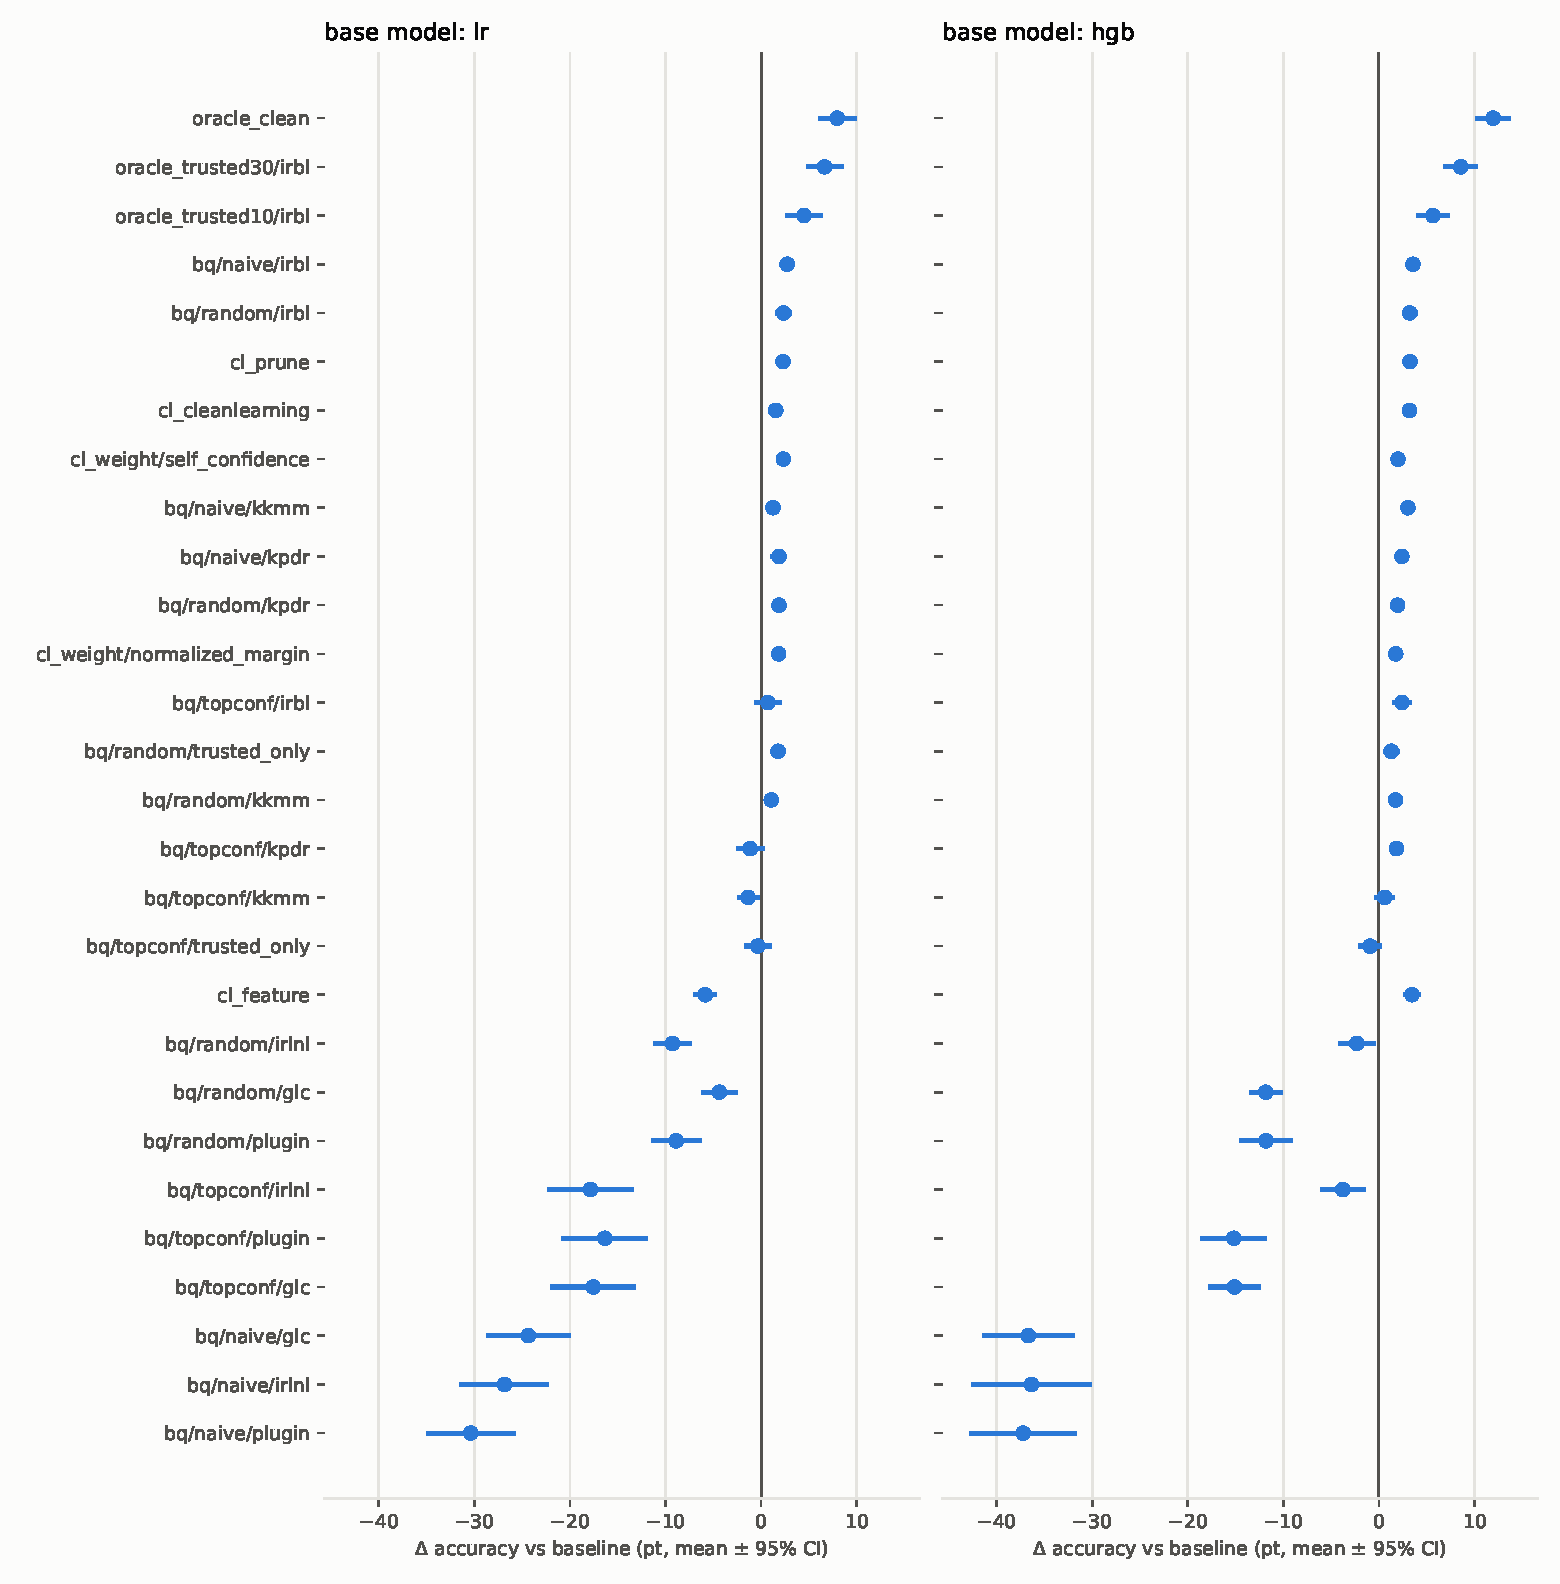
\includegraphics[width=\textwidth]{figures/delta_vs_baseline.pdf}
  \caption{\method{baseline} に対する精度差の平均と 95\% 信頼区間（左：LR、右：HGB）。}
  \label{fig:delta}
\end{figure}

\subsection{手法間の対比較}
表~\ref{tab:paired} に、同一条件どうしの精度差を示す。
\method{bq/naive/irbl} は \method{cl\_prune} を平均で LR \PLRNaiveIrblVsPrune{}、HGB \PHGBNaiveIrblVsPrune{}~pt 上回り、勝率はそれぞれ \PLRNaiveIrblVsPruneWin\%、\PHGBNaiveIrblVsPruneWin\% であった。
差は小さいが、信頼区間は両モデルとも 0 を含まない。
学習時間は \method{cl\_prune} の LR で \TimeLRRatio{} 倍、HGB で \TimeHGBRatio{} 倍であった。

\method{cl\_cleanlearning} は \method{cl\_prune} に対して LR で \PLRCLVsPrune{}~pt（勝率 \PLRCLVsPruneWin\%）、HGB で \PHGBCLVsPrune{}~pt（勝率 \PHGBCLVsPruneWin\%）であった。
クラスごとの再重み付けは、LR では精度を下げ、HGB ではほぼ影響しなかった。
このため \method{bq/naive/irbl} と \method{cl\_cleanlearning} の差（LR \PLRNaiveIrblVsCL{}、HGB \PHGBNaiveIrblVsCL{}~pt）は、\method{cl\_prune} との差より大きい。

分割方式の間では、\method{random} が \method{topconf} を一貫して上回った（IRBL で LR \PLRRandomIrblVsTopIrbl{}、HGB \PHGBRandomIrblVsTopIrbl{}~pt、\method{trusted\_only} で LR \PLRRandomTVsTopT{}、HGB \PHGBRandomTVsTopT{}~pt）。
\method{naive} は \method{random} をわずかに上回った（IRBL で LR \PLRNaiveIrblVsRandomIrbl{}、HGB \PHGBNaiveIrblVsRandomIrbl{}~pt）。
各分割で $\mathcal{T}$ のみの学習に対する IRBL の上積みを見ると、\method{random} では LR \PLRRandomIrblVsRandomT{}、HGB \PHGBRandomIrblVsRandomT{}~pt であり、\method{naive} での上積み（\method{cl\_prune} に対する差）より大きい。
すなわち \method{naive} の優位は IRBL の重み付けの効果というより、$\mathcal{T}$ が大きいことによる部分が大きい（\ref{sec:discussion} 節）。

品質スコアを重みにする \method{cl\_weight/self\_confidence} は、LR では \method{cl\_prune} と同程度（\PLRWeightVsPrune）、HGB では劣った（\PHGBWeightVsPrune）。
特徴量にする \method{cl\_feature} は、HGB では \method{cl\_prune} と同程度（\PHGBFeatureVsPrune）であったが、LR では大きく劣った（\PLRFeatureVsPrune）。

\begin{table}[tbp]
  \centering
  \caption{同一条件における手法 A と手法 B の精度差（pt）。勝率は A が B を上回った条件の割合（\%）。差は丸める前の精度から計算しているため、表~\ref{tab:overall} の丸めた値どうしの差と 0.01~pt ずれることがある。}
  \label{tab:paired}
  \footnotesize
  \setlength{\tabcolsep}{4pt}
  \begin{tabular}{llrrrr}
\toprule
 & & \multicolumn{2}{c}{LR} & \multicolumn{2}{c}{HGB} \\
\cmidrule(lr){3-4} \cmidrule(lr){5-6}
手法 A & 手法 B & A$-$B (95\% CI) & A 勝率 & A$-$B (95\% CI) & A 勝率 \\
\midrule
\texttt{bq/naive/irbl} & \texttt{cl\_prune} & +0.45 {\scriptsize$\pm$0.36} & 64 & +0.31 {\scriptsize$\pm$0.24} & 71 \\
\texttt{bq/naive/irbl} & \texttt{cl\_cleanlearning} & +1.20 {\scriptsize$\pm$0.40} & 76 & +0.37 {\scriptsize$\pm$0.24} & 72 \\
\texttt{cl\_cleanlearning} & \texttt{cl\_prune} & $-$0.75 {\scriptsize$\pm$0.22} & 17 & $-$0.06 {\scriptsize$\pm$0.17} & 37 \\
\texttt{bq/random/irbl} & \texttt{bq/random/trusted\_only} & +0.58 {\scriptsize$\pm$0.27} & 80 & +1.91 {\scriptsize$\pm$0.33} & 88 \\
\texttt{bq/naive/irbl} & \texttt{bq/random/irbl} & +0.38 {\scriptsize$\pm$0.24} & 66 & +0.34 {\scriptsize$\pm$0.28} & 68 \\
\texttt{bq/random/irbl} & \texttt{bq/topconf/irbl} & +1.65 {\scriptsize$\pm$0.76} & 72 & +0.80 {\scriptsize$\pm$0.35} & 69 \\
\texttt{bq/random/trusted\_only} & \texttt{bq/topconf/trusted\_only} & +2.13 {\scriptsize$\pm$0.85} & 70 & +2.24 {\scriptsize$\pm$0.50} & 86 \\
\texttt{cl\_weight/self\_confidence} & \texttt{cl\_prune} & +0.04 {\scriptsize$\pm$0.28} & 57 & $-$1.26 {\scriptsize$\pm$0.47} & 30 \\
\texttt{cl\_feature} & \texttt{cl\_prune} & $-$8.14 {\scriptsize$\pm$1.14} & 2 & +0.21 {\scriptsize$\pm$0.50} & 47 \\
\texttt{oracle\_trusted10/irbl} & \texttt{bq/naive/irbl} & +1.75 {\scriptsize$\pm$1.32} & 41 & +2.08 {\scriptsize$\pm$1.29} & 44 \\
\texttt{oracle\_trusted30/irbl} & \texttt{bq/naive/irbl} & +3.91 {\scriptsize$\pm$1.35} & 72 & +5.00 {\scriptsize$\pm$1.38} & 92 \\
\texttt{oracle\_trusted30/irbl} & \texttt{oracle\_trusted10/irbl} & +2.16 {\scriptsize$\pm$0.32} & 99 & +2.92 {\scriptsize$\pm$0.58} & 96 \\
\bottomrule
\end{tabular}

\end{table}

\subsection{ノイズの種類による違い}
表~\ref{tab:noise} にノイズの種類と率ごとの $\Delta$ を示す。
自動の手法による改善が最も大きかったのは pair ノイズであり、ノイズ率 40\% で \method{bq/naive/irbl} は LR +6.91、HGB +7.48~pt であった。
ただし同じ条件で \method{oracle\_trusted10/irbl} は LR +19.94、HGB +21.40~pt、\method{oracle\_trusted30/irbl} は LR +21.95、HGB +24.22~pt であり、人手で確認したサンプルを trusted とすることの効果が非常に大きかった。
instance ノイズでは自動の手法の改善は小さく、LR ではどの手法も 1~pt 以下であった。
LR の instance 40\% では \method{bq/naive/irbl}（$-$0.18）が \method{cl\_prune}（+0.76）を下回った（理由は \ref{sec:mech} 節）。
\method{cl\_cleanlearning} の \method{cl\_prune} に対する劣後は LR の symmetric ノイズで最も大きかった（40\% で +0.68 対 +2.21）。

全体平均では \method{oracle\_trusted10/irbl} が \method{bq/naive/irbl} を上回るものの、条件ごとの勝率は LR \PLROracleTenVsNaiveIrblWin\%、HGB \PHGBOracleTenVsNaiveIrblWin\% と半数に満たず、平均の差の大部分は pair ノイズ 40\% によるものである。
一方、trusted の大きさを 30\% にそろえた \method{oracle\_trusted30/irbl} は、\method{bq/naive/irbl} を LR \PLROracleThirtyVsNaiveIrbl{}~pt（勝率 \PLROracleThirtyVsNaiveIrblWin\%）、HGB \PHGBOracleThirtyVsNaiveIrbl{}~pt（勝率 \PHGBOracleThirtyVsNaiveIrblWin\%）上回った。
10\% から 30\% への増加は、ほぼすべての条件で精度を上げた（勝率 LR \PLROracleThirtyVsOracleTenWin\%、HGB \PHGBOracleThirtyVsOracleTenWin\%）。

\begin{table}[tbp]
  \centering
  \caption{ノイズの種類と率ごとの $\Delta$（pt、3 データセット $\times$ 5 シードの平均）。主要な手法のみ。先頭行は \method{baseline} の精度（\%）。全手法は付録の表~\ref{tab:noise-all}。}
  \label{tab:noise}
  \footnotesize
  \begin{tabular}{lrrrrrr}
\toprule
\multicolumn{7}{l}{\textbf{LR}} \\
 & \multicolumn{2}{c}{symmetric} & \multicolumn{2}{c}{pair} & \multicolumn{2}{c}{instance} \\
\cmidrule(lr){2-3} \cmidrule(lr){4-5} \cmidrule(lr){6-7}
 & 20\% & 40\% & 20\% & 40\% & 20\% & 40\% \\
\midrule
\textit{baseline 精度 (\%)} & 77.91 & 75.63 & 73.27 & 58.20 & 78.35 & 75.51 \\
\addlinespace
\texttt{oracle\_clean} & +3.19 & +5.47 & +7.83 & +22.90 & +2.74 & +5.58 \\
\texttt{oracle\_trusted10/irbl} & +0.25 & +2.26 & +5.36 & +19.94 & $-$1.33 & +0.39 \\
\texttt{oracle\_trusted30/irbl} & +2.33 & +4.37 & +7.17 & +21.95 & +1.07 & +2.93 \\
\texttt{cl\_prune} & +1.61 & +2.21 & +4.54 & +3.87 & +0.70 & +0.76 \\
\texttt{cl\_cleanlearning} & +0.64 & +0.68 & +4.17 & +2.92 & +0.46 & +0.30 \\
\texttt{bq/naive/irbl} & +1.92 & +2.16 & +5.37 & +6.91 & +0.19 & $-$0.18 \\
\texttt{bq/random/irbl} & +1.83 & +2.15 & +5.25 & +5.33 & +0.04 & $-$0.50 \\
\texttt{bq/topconf/irbl} & $-$0.38 & +0.14 & +3.01 & +3.26 & $-$1.12 & $-$0.73 \\
\texttt{bq/naive/kpdr} & +0.86 & +0.74 & +4.39 & +5.77 & $-$0.48 & $-$0.18 \\
\texttt{cl\_weight/self\_confidence} & +2.31 & +2.98 & +3.78 & +3.17 & +1.00 & +0.67 \\
\texttt{cl\_feature} & $-$5.31 & $-$10.40 & $-$6.07 & $-$8.97 & $-$1.66 & $-$2.76 \\
\texttt{bq/random/glc} & $-$7.05 & $-$6.73 & $-$1.49 & $-$8.55 & $-$1.59 & $-$0.78 \\
\texttt{bq/naive/glc} & $-$38.60 & $-$32.27 & $-$32.78 & $-$25.11 & $-$9.75 & $-$7.66 \\
\midrule
\multicolumn{7}{l}{\textbf{HGB}} \\
 & \multicolumn{2}{c}{symmetric} & \multicolumn{2}{c}{pair} & \multicolumn{2}{c}{instance} \\
\cmidrule(lr){2-3} \cmidrule(lr){4-5} \cmidrule(lr){6-7}
 & 20\% & 40\% & 20\% & 40\% & 20\% & 40\% \\
\midrule
\textit{baseline 精度 (\%)} & 85.61 & 78.68 & 82.35 & 61.36 & 81.64 & 71.91 \\
\addlinespace
\texttt{oracle\_clean} & +3.26 & +10.19 & +6.52 & +27.51 & +7.23 & +16.96 \\
\texttt{oracle\_trusted10/irbl} & $-$0.45 & +4.44 & +2.61 & +21.40 & +0.15 & +5.68 \\
\texttt{oracle\_trusted30/irbl} & +1.68 & +6.69 & +4.18 & +24.22 & +3.69 & +10.90 \\
\texttt{cl\_prune} & +0.51 & +5.23 & +2.99 & +7.13 & +0.46 & +3.19 \\
\texttt{cl\_cleanlearning} & +0.46 & +5.07 & +2.85 & +6.70 & +0.83 & +3.23 \\
\texttt{bq/naive/irbl} & +1.29 & +5.27 & +3.73 & +7.48 & +0.92 & +2.67 \\
\texttt{bq/random/irbl} & +0.76 & +4.85 & +3.19 & +7.36 & +0.23 & +2.93 \\
\texttt{bq/topconf/irbl} & $-$0.55 & +4.11 & +2.09 & +7.06 & $-$0.83 & +2.61 \\
\texttt{bq/naive/kpdr} & +0.72 & +3.14 & +2.89 & +6.06 & $-$0.18 & +1.74 \\
\texttt{cl\_weight/self\_confidence} & +0.88 & +3.61 & +2.16 & +3.09 & +0.78 & +1.43 \\
\texttt{cl\_feature} & $-$0.46 & +4.51 & +2.63 & +9.97 & +0.34 & +3.74 \\
\texttt{bq/random/glc} & $-$11.19 & $-$18.30 & $-$16.12 & $-$15.62 & $-$6.65 & $-$3.18 \\
\texttt{bq/naive/glc} & $-$53.12 & $-$40.74 & $-$52.48 & $-$26.30 & $-$26.29 & $-$21.20 \\
\bottomrule
\end{tabular}

\end{table}

\subsection{\cl{} の検出性能と分割の質}\label{sec:diag}
表~\ref{tab:diag} に \cl{} の検出性能と、各分割における誤ラベル率を示す。
symmetric と pair 20\% では再現率が 84--91\% と高いのに対し、instance ノイズでは \InstRecallMin--\InstRecallMax\%（データセット・モデル別の平均の範囲）にとどまった。
\method{naive} の untrusted（=誤り判定サンプル）の誤ラベル率は \NaiveUntrustedMin--\NaiveUntrustedMax\% であり、\method{naive} の trusted にも条件によって 2--26\% の誤ラベルが残った。
\method{random} と \method{topconf} の untrusted の誤ラベル率も、$\mathcal{I}$ がすべて untrusted に入るため $\rho$ より高い（$\rho = 20\%$ で 23--28\%、$\rho = 40\%$ で 45--54\%）。
\method{topconf} の trusted は \method{random} の trusted より誤ラベル率が低い（たとえば HGB の symmetric 20\% で 1.2\% 対 3.1\%）。
それにもかかわらず、前節のとおり精度では \method{random} が上回った。

\begin{table}[tbp]
  \centering
  \caption{\cl{} の検出性能と疑似分割の誤ラベル率（\%、3 データセット $\times$ 5 シードの平均）。指摘率は誤り判定を受けたサンプルの割合。T は trusted、U は untrusted。\method{naive} では $\mathcal{U} = \mathcal{I}$ のため naive U の誤ラベル率は適合率に等しく、naive T の大きさは 1 $-$ 指摘率である。}
  \label{tab:diag}
  \footnotesize
  \setlength{\tabcolsep}{3.5pt}
  \begin{tabular}{lllrrrrrrrrr}
\toprule
 & & & \multicolumn{3}{c}{cleanlab の検出} & \multicolumn{2}{c}{naive} & \multicolumn{2}{c}{random} & \multicolumn{2}{c}{topconf} \\
\cmidrule(lr){4-6} \cmidrule(lr){7-8} \cmidrule(lr){9-10} \cmidrule(lr){11-12}
モデル & ノイズ & 率 & 指摘率 & 適合率 & 再現率 & T & U & T & U & T & U \\
\midrule
LR & symmetric & 20\% & 28.8 & 62.9 & 88.2 & 3.4 & 62.9 & 4.2 & 26.6 & 1.7 & 27.6 \\
 & symmetric & 40\% & 42.6 & 80.1 & 85.0 & 10.4 & 80.1 & 12.2 & 51.3 & 5.7 & 53.9 \\
 & pair & 20\% & 31.3 & 53.9 & 83.7 & 4.8 & 53.9 & 5.6 & 26.0 & 2.6 & 27.3 \\
 & pair & 40\% & 45.1 & 58.1 & 65.4 & 25.2 & 58.1 & 27.9 & 45.1 & 23.3 & 47.0 \\
 & instance & 20\% & 18.7 & 55.5 & 48.7 & 12.7 & 55.5 & 13.0 & 23.0 & 4.8 & 26.5 \\
 & instance & 40\% & 27.8 & 78.9 & 55.6 & 24.4 & 78.9 & 25.3 & 46.3 & 11.1 & 52.4 \\
\addlinespace
HGB & symmetric & 20\% & 26.0 & 71.8 & 91.4 & 2.4 & 71.8 & 3.1 & 27.1 & 1.2 & 27.9 \\
 & symmetric & 40\% & 44.4 & 79.9 & 88.6 & 8.2 & 79.9 & 10.2 & 52.4 & 5.6 & 54.3 \\
 & pair & 20\% & 27.6 & 63.2 & 86.4 & 3.8 & 63.2 & 5.2 & 26.3 & 2.5 & 27.4 \\
 & pair & 40\% & 45.7 & 56.3 & 64.3 & 26.2 & 56.3 & 28.2 & 45.1 & 23.4 & 47.1 \\
 & instance & 20\% & 20.7 & 61.4 & 61.0 & 9.9 & 61.4 & 9.9 & 24.3 & 3.4 & 27.1 \\
 & instance & 40\% & 30.7 & 73.0 & 56.2 & 25.2 & 73.0 & 26.5 & 45.8 & 14.7 & 50.8 \\
\bottomrule
\end{tabular}

\end{table}

\subsection{対照実験：本物の trusted を与えた場合}\label{sec:oracle}
疑似 trusted に起因する劣化と手法自体の性能とを切り分けるため、一様無作為に選んだ 10\% または 30\% のサンプルのラベルを真のラベルに戻して trusted とし、同じアルゴリズムを評価した（表~\ref{tab:oracle}）。
重み付け系の IRBL と K-PDR は oracle で最もよく、naive・random でも正の改善を保った。
\method{trusted\_only} は oracle 10\% では HGB で \OHGBTRUSTEDONLYTen{} にとどまったが、30\% では LR \OLRTRUSTEDONLYThirty{}、HGB \OHGBTRUSTEDONLYThirty{} となり、trusted の大きさが結果を大きく左右した。

遷移行列系は oracle でも多くの場合 \method{baseline} を下回った（GLC は 10\% で LR \OLRGLCTen{}、HGB \OHGBGLCTen{}、30\% で LR \OLRGLCThirty{}、HGB \OHGBGLCThirty{}）。
例外は HGB の IRLNL で、30\% では \OHGBIRLNLThirty{} と改善した。
ただし \method{naive} での劣化（$-$24～$-$37~pt）は oracle よりはるかに大きかった。
すなわち、遷移行列系は本実験の設定ではそもそも強くなく、疑似 trusted がそれをさらに大きく悪化させた。

遷移行列系が oracle でも弱い理由として、当初は trusted の少ない少数クラス（covtype）での推定の不安定さを想定した。
データセット別の内訳（表~\ref{tab:oracle-breakdown}）を見ると、Plugin の劣化は covtype に集中しており（LR で $-$20~pt 前後）、この仮説と整合する。
一方、GLC と IRLNL はクラス比の釣り合った synth でも LR で劣化し（GLC は最大 $-$4.3~pt、IRLNL は symmetric・instance で $-$18～$-$24~pt）、少数クラスだけでは説明できない。
GLC の対角成分の推定は trusted を 10\% から 30\% に増やしてもほとんど変わらなかった（\ref{sec:mech} 節）ことから、件数よりも推定の偏りが主な要因と考えられる。

\begin{table}[tbp]
  \centering
  \caption{trusted の作り方による $\Delta$（pt）の比較。naive・random は \cl{} による疑似 trusted、oracle10・oracle30 は一様無作為に選んだ 10\%・30\% を真のラベルに戻した本物の trusted。$^\dagger$ \method{bq/naive/trusted\_only} は \method{cl\_prune} と同一のため、その値を示した。}
  \label{tab:oracle}
  \footnotesize
  \begin{tabular}{lrrrrrrrr}
\toprule
 & \multicolumn{4}{c}{LR} & \multicolumn{4}{c}{HGB} \\
\cmidrule(lr){2-5} \cmidrule(lr){6-9}
アルゴリズム & naive & random & oracle10 & oracle30 & naive & random & oracle10 & oracle30 \\
\midrule
\texttt{trusted\_only} & +2.28$^\dagger$ & +1.77 & +3.45 & +6.47 & +3.25$^\dagger$ & +1.31 & $-$0.16 & +6.81 \\
\texttt{irbl} & +2.73 & +2.35 & +4.48 & +6.64 & +3.56 & +3.22 & +5.64 & +8.56 \\
\texttt{kpdr} & +1.85 & +1.86 & +3.11 & +6.14 & +2.40 & +1.95 & +4.49 & +7.17 \\
\texttt{glc} & $-$24.36 & $-$4.37 & $-$2.62 & $-$0.85 & $-$36.69 & $-$11.84 & $-$11.78 & $-$6.06 \\
\texttt{plugin} & $-$30.37 & $-$8.89 & $-$2.97 & $-$3.58 & $-$37.23 & $-$11.81 & $-$2.46 & $-$2.23 \\
\texttt{irlnl} & $-$26.86 & $-$9.27 & $-$10.82 & $-$8.93 & $-$36.34 & $-$2.32 & $-$1.31 & +5.08 \\
\bottomrule
\end{tabular}

\end{table}

\begin{table}[tbp]
  \centering
  \caption{本物の trusted を与えた場合の $\Delta$（pt）のデータセット・ノイズ別の内訳（2 ノイズ率 $\times$ 5 シードの平均）。sym = symmetric、inst = instance。}
  \label{tab:oracle-breakdown}
  \scriptsize
  \setlength{\tabcolsep}{3.5pt}
  \begin{tabular}{llrrrrrrrrr}
\toprule
 & & \multicolumn{3}{c}{covtype} & \multicolumn{3}{c}{digits} & \multicolumn{3}{c}{synth} \\
\cmidrule(lr){3-5} \cmidrule(lr){6-8} \cmidrule(lr){9-11}
アルゴリズム & trusted & sym & pair & inst & sym & pair & inst & sym & pair & inst \\
\midrule
\multicolumn{11}{l}{\textbf{LR}} \\
\texttt{irbl} & 10\% & $-$0.4 & +3.3 & $-$2.1 & +4.7 & +23.2 & +2.9 & $-$0.6 & +11.4 & $-$2.2 \\
 & 30\% & +1.2 & +5.0 & $-$0.2 & +8.0 & +25.9 & +6.5 & +0.9 & +12.7 & $-$0.3 \\
\texttt{glc} & 10\% & $-$4.6 & $-$5.1 & $-$5.1 & +0.2 & +0.4 & +0.2 & $-$4.3 & $-$1.7 & $-$3.6 \\
 & 30\% & $-$10.1 & $-$2.7 & $-$3.5 & +2.3 & +10.2 & +2.4 & $-$3.4 & +0.0 & $-$2.8 \\
\texttt{plugin} & 10\% & $-$19.6 & $-$8.2 & $-$2.7 & $-$1.5 & +2.9 & $-$0.3 & $-$0.7 & +3.7 & $-$0.2 \\
 & 30\% & $-$20.2 & $-$8.7 & $-$2.3 & $-$4.4 & +3.6 & $-$2.1 & $-$1.0 & +3.2 & $-$0.2 \\
\texttt{irlnl} & 10\% & $-$4.5 & $-$11.5 & $-$7.9 & $-$13.2 & $-$0.8 & $-$3.0 & $-$21.2 & $-$11.6 & $-$23.7 \\
 & 30\% & $-$10.1 & $-$11.4 & $-$6.5 & $-$11.3 & +6.4 & $-$1.3 & $-$19.1 & $-$8.9 & $-$18.1 \\
\midrule\multicolumn{11}{l}{\textbf{HGB}} \\
\texttt{irbl} & 10\% & $-$1.9 & +6.1 & $-$0.8 & +4.2 & +16.2 & +3.9 & +3.6 & +13.7 & +5.6 \\
 & 30\% & +0.9 & +7.3 & +4.1 & +5.5 & +19.1 & +8.4 & +6.1 & +16.1 & +9.3 \\
\texttt{glc} & 10\% & $-$14.6 & $-$20.5 & $-$12.5 & $-$12.4 & $-$11.5 & $-$9.5 & $-$5.2 & $-$10.6 & $-$9.1 \\
 & 30\% & $-$9.2 & $-$8.0 & $-$8.2 & $-$6.7 & $-$2.1 & $-$4.2 & $-$3.0 & $-$7.0 & $-$6.1 \\
\texttt{plugin} & 10\% & $-$9.5 & $-$10.6 & $-$6.0 & $-$0.4 & +2.2 & $-$0.6 & $-$0.9 & +3.8 & $-$0.1 \\
 & 30\% & $-$8.6 & $-$4.4 & $-$1.5 & $-$2.9 & $-$0.7 & $-$1.6 & $-$2.3 & +2.2 & $-$0.3 \\
\texttt{irlnl} & 10\% & $-$1.7 & $-$16.5 & $-$13.1 & +2.2 & +4.8 & +1.9 & +2.5 & +5.6 & +2.5 \\
 & 30\% & +0.1 & +3.9 & +2.0 & +4.1 & +11.5 & +4.8 & +3.9 & +10.2 & +5.2 \\
\bottomrule
\end{tabular}

\end{table}

\subsection{メカニズムの分析}\label{sec:mech}
全 \NCond{} 条件と両モデルについて、GLC が推定した遷移行列（表~\ref{tab:mech-glc}）と、IRBL が untrusted に付けた重み（表~\ref{tab:mech-irbl}）を調べた。

\paragraph{遷移行列の推定}
真の遷移行列の対角成分の平均は \MechLRTrueDiag{} であるのに対し、\method{naive} から推定した値は LR で \MechLRNaiveDiag{}、HGB で \MechHGBNaiveDiag{} であった。
\texttt{gold} 推定は $\mathcal{U}$ で学習した分類器を用いるため、推定値が反映するのはデータ全体ではなく $\mathcal{U}$ のノイズである。
\method{naive} の $\mathcal{U}$ で正しいラベルの割合は LR で \MechLRNaiveUClean{}、HGB で \MechHGBNaiveUClean{} しかなく、推定値はそれをさらに下回った。
$\mathcal{U} = \mathcal{I}$ はモデルの予測と観測ラベルが食い違ったサンプルだけからなるため、$\mathcal{U}$ で学習した分類器は $\mathcal{T}$ のラベルとは逆の対応を学びやすい。
このためノイズが実際より大幅に多いと推定され、その補正が予測を誤った方向へ書き換えたと考えられる。
\method{random} では $\mathcal{U}$ に誤り判定のないサンプルが混ざることで $\mathcal{U}$ の正ラベル率が \MechLRRandomUClean{} に上がり、推定値も LR \MechLRRandomDiag{}、HGB \MechHGBRandomDiag{} に改善した。

本物の trusted を与えても、推定値は $\mathcal{U}$ の正ラベル率（\MechLROracleTenUClean{}）を下回った（LR で \MechLROracleTenDiag{}、HGB で \MechHGBOracleTenDiag{}）。
trusted を 30\% にしても推定値はほぼ変わらなかった（LR \MechLROracleThirtyDiag{}、HGB \MechHGBOracleThirtyDiag{}）。
\texttt{gold} 推定は、$\mathcal{U}$ で学習した分類器がノイズ付きラベルの事後確率を正確に表すことを前提とする。
分類器の予測確率が真のクラスに集中しないと、ノイズがなくても対角成分は 1 より小さく推定されるため、分類器自身の誤差がノイズとして上乗せされると考えられる。
LR で過小推定が大きく、表現力の高い HGB で小さいことはこの解釈と整合する。
ただし HGB では推定値が真値に近いにもかかわらず GLC の精度低下は LR より大きく（表~\ref{tab:oracle}）、推定のずれだけでは説明できない。
補正後の学習との相互作用など別の要因があると考えられるが、本研究では特定していない。

\paragraph{IRBL の重み}
IRBL は \method{naive} の untrusted のうち、実際に誤ったラベルに平均 LR \MechLRWNoisy{}・HGB \MechHGBWNoisy{}、実際には正しいラベルに平均 LR \MechLRWClean{}・HGB \MechHGBWClean{} の重みを付けた。
つまり IRBL は誤り判定サンプルを一律に捨てるのではなく、\cl{} の誤検出（正しいのに誤りと判定されたサンプル）を拾い直していた。
これが \method{cl\_prune} に対するわずかな優位の理由と考えられる。
重みの絶対値はモデルによって異なるが、正しいラベルと誤ったラベルの重みの比は \method{naive}（LR 6.1 倍、HGB 5.6 倍）、\method{random}（3.4 倍、4.9 倍）、\method{topconf}（2.6 倍、4.1 倍）の順に小さくなった。
\method{topconf} では trusted が簡単なサンプルに偏るため、IRBL が誤ラベルと「難しいが正しいラベル」を区別しにくくなったと考えられ、RQ2 の結果と整合する。

LR の instance 40\% では、\method{naive} の untrusted の誤ったラベルに付いた重みは平均 0.80 であり、symmetric（0.04--0.09）と比べてほとんど下がらなかった。
instance ノイズは LR にとって自然に見える誤りであり、\method{naive} の trusted にも 24\% の誤ラベルが残るため、IRBL は誤りを見分けられない。
これが同条件で \method{bq/naive/irbl} が \method{cl\_prune} を下回った理由と考えられる。

\begin{table}[tbp]
  \centering
  \caption{GLC（\texttt{gold}）が推定した遷移行列の対角成分の平均と、untrusted の正しいラベルの割合（3 データセット $\times$ 5 シードの平均）。真値はデータ全体の真の遷移行列の対角成分をクラスについて単純平均した値 $\frac{1}{K}\sum_{k} T_{kk}$ である。instance ノイズでは誤りやすいクラスに反転が偏るため、サンプル単位のノイズ率 $\rho$ とは一致しない。}
  \label{tab:mech-glc}
  \scriptsize
  \setlength{\tabcolsep}{3.5pt}
  \begin{tabular}{lllrrrrrrrrr}
\toprule
 & & & \multicolumn{5}{c}{GLC が推定した対角平均} & \multicolumn{3}{c}{U の正ラベル率} \\
\cmidrule(lr){4-8} \cmidrule(lr){9-11}
モデル & ノイズ & 率 & 真値 & naive & random & topconf & oracle10 & oracle30 & naive & random & oracle10 \\
\midrule
LR & symmetric & 20\% & 0.80 & 0.12 & 0.42 & 0.47 & 0.49 & 0.49 & 0.37 & 0.73 & 0.80 \\
 & symmetric & 40\% & 0.60 & 0.10 & 0.27 & 0.24 & 0.37 & 0.37 & 0.20 & 0.49 & 0.60 \\
 & pair & 20\% & 0.80 & 0.19 & 0.47 & 0.53 & 0.50 & 0.49 & 0.46 & 0.74 & 0.80 \\
 & pair & 40\% & 0.60 & 0.25 & 0.37 & 0.39 & 0.38 & 0.38 & 0.42 & 0.55 & 0.60 \\
 & instance & 20\% & 0.78 & 0.34 & 0.68 & 0.80 & 0.65 & 0.64 & 0.45 & 0.77 & 0.80 \\
 & instance & 40\% & 0.57 & 0.36 & 0.64 & 0.75 & 0.60 & 0.60 & 0.21 & 0.54 & 0.60 \\
\addlinespace
HGB & symmetric & 20\% & 0.80 & 0.11 & 0.61 & 0.66 & 0.68 & 0.68 & 0.28 & 0.73 & 0.80 \\
 & symmetric & 40\% & 0.60 & 0.11 & 0.39 & 0.38 & 0.53 & 0.53 & 0.20 & 0.48 & 0.60 \\
 & pair & 20\% & 0.80 & 0.14 & 0.62 & 0.68 & 0.67 & 0.66 & 0.37 & 0.74 & 0.80 \\
 & pair & 40\% & 0.60 & 0.28 & 0.45 & 0.44 & 0.49 & 0.49 & 0.44 & 0.55 & 0.60 \\
 & instance & 20\% & 0.78 & 0.31 & 0.76 & 0.84 & 0.72 & 0.71 & 0.39 & 0.76 & 0.80 \\
 & instance & 40\% & 0.57 & 0.31 & 0.69 & 0.77 & 0.63 & 0.63 & 0.27 & 0.54 & 0.60 \\
\bottomrule
\end{tabular}

\end{table}

\begin{table}[tbp]
  \centering
  \caption{IRBL が untrusted に付けた重みの平均（3 データセット $\times$ 5 シードの平均）。誤・正は、untrusted のうち実際に誤ったラベル・正しいラベルのサンプル。}
  \label{tab:mech-irbl}
  \footnotesize
  \begin{tabular}{lllrrrrrr}
\toprule
 & & & \multicolumn{2}{c}{naive} & \multicolumn{2}{c}{random} & \multicolumn{2}{c}{topconf} \\
\cmidrule(lr){4-5} \cmidrule(lr){6-7} \cmidrule(lr){8-9}
モデル & ノイズ & 率 & 誤 & 正 & 誤 & 正 & 誤 & 正 \\
\midrule
LR & symmetric & 20\% & 0.04 & 1.48 & 0.14 & 1.42 & 0.33 & 1.35 \\
 & symmetric & 40\% & 0.09 & 2.32 & 0.19 & 2.04 & 0.29 & 1.96 \\
 & pair & 20\% & 0.06 & 2.07 & 0.18 & 1.38 & 0.31 & 1.36 \\
 & pair & 40\% & 0.25 & 1.81 & 0.49 & 1.33 & 0.52 & 1.26 \\
 & instance & 20\% & 0.65 & 1.29 & 0.72 & 1.04 & 0.85 & 1.05 \\
 & instance & 40\% & 0.80 & 2.53 & 0.74 & 1.17 & 0.83 & 1.21 \\
\addlinespace
HGB & symmetric & 20\% & 0.01 & 0.36 & 0.03 & 0.91 & 0.05 & 0.82 \\
 & symmetric & 40\% & 0.02 & 0.53 & 0.05 & 0.98 & 0.06 & 0.92 \\
 & pair & 20\% & 0.02 & 0.46 & 0.07 & 0.89 & 0.09 & 0.81 \\
 & pair & 40\% & 0.17 & 0.54 & 0.28 & 0.75 & 0.28 & 0.70 \\
 & instance & 20\% & 0.12 & 0.37 & 0.31 & 0.87 & 0.36 & 0.80 \\
 & instance & 40\% & 0.15 & 0.48 & 0.35 & 0.90 & 0.35 & 0.86 \\
\bottomrule
\end{tabular}

\end{table}

\section{考察}\label{sec:discussion}

\paragraph{RQ1：疑似バイクオリティ化は除去より良いか}
重み付け系、特に IRBL と組み合わせた場合に限り、除去をわずかに上回った。
改善幅は 0.3--0.5~pt と小さく、学習時間は約 3 倍となる。
\cl{} 標準の \texttt{CleanLearning} は除去されるサンプルが同一でクラスごとの再重み付けを加えるだけだが、\method{cl\_prune} を上回らなかった。
ノイズ率がクラスによらない symmetric ノイズで LR の劣後が最も大きかったことから、推定されたクラス別ノイズ率のばらつきが不要なクラス間の偏りを持ち込んだ可能性がある。
したがって、\method{bq/naive/irbl} の優位は再重み付けの有無では説明できず、誤検出されたサンプルを個別に拾い直す点にあると考えられる。

ただし、\method{naive} の優位には trusted の大きさも寄与している。
\method{naive} の $\mathcal{T}$ は学習データの過半を占めるのに対し、\method{random} は約 30\% である。
$\mathcal{T}$ のみの学習に対する IRBL の上積みは \method{random} の方が大きかったことから、IRBL の重み付け自体は小さい $\mathcal{T}$ でも機能し、\method{naive} の利点は主に $\mathcal{T}$ の大きさにあると考えられる。
遷移行列系との組み合わせは避けるべきである。

\paragraph{RQ2：trusted の選び方}
品質スコアの上位を trusted とする \method{topconf} は、trusted の誤ラベル率を下げたにもかかわらず精度を下げた。
trusted が「モデルにとって簡単なサンプル」に偏ると、重み付け系は「簡単か難しいか」を手がかりに重みを付けてしまい、難しいが正しいサンプルの重みが下がると考えられる。
IRBL の重みの実測（表~\ref{tab:mech-irbl}）もこれを支持する。
確信度による選別が学習しやすいサンプルに偏り、曖昧なサンプルが汎化に寄与するという Dataset Cartography~\cite{swayamdipta2020cartography} の知見とも整合する。
疑似 trusted を作る際は、ラベルのきれいさよりも、untrusted と同じ分布に従うことを優先すべきである。

ただしこの傾向はデータセットに依存した（付録の表~\ref{tab:dataset-all}）。
クラス比の偏りが大きい covtype の LR では、学習データの 30\% に絞る分割はいずれも \method{baseline} を下回り（\method{bq/random/irbl} $-$0.53、\method{bq/random/trusted\_only} $-$1.14~pt）、正の改善は \method{bq/naive/irbl}（+0.53）と \method{cl\_prune}（+0.14）に限られた。
一方 digits の LR では \method{bq/topconf/irbl}（+7.01）が \method{bq/random/irbl}（+5.41）を上回った。
trusted を絞ることの不利と選択バイアスの影響は、データの構造やクラス比と相互作用すると考えられる。

\paragraph{RQ3：品質スコアの重み・特徴量としての利用}
重みとしての利用は除去と同等か劣り、利点は見られなかった。
特徴量としての利用は HGB では除去と同程度に機能したが、LR では大きく劣化した。
これには 3 つの要因が考えられる。
第 1 に、多クラスのロジスティック回帰に $s$ を加法的に結合すると、クラス $c$ のロジットは $w_c^\top x + w_{c,s} s + b_c$ となり、$s$ はロジットを $x$ と無関係にずらすことしかできない。
このため「ラベルが信頼できるときの決定境界」を表現できない。
これは交互作用項（$s x$ など）を持たない加法的な結合に固有の制約であり、交互作用を明示的に加えれば線形モデルでも表現できる。
第 2 に、学習時の $s$ は 1 より小さい値に広く分布するのに対し、推論時には一律に $s=1$ を与える。
学習時に平均的な $s$ の高いクラスに正の $w_{c,s}$ が付くと、推論時には $w_{c,s}(1 - \bar{s})$ に相当する定数がクラスごとの切片に加わり、予測がそれらのクラスへ偏る可能性がある。
LR が symmetric ノイズでも大きく劣化した（20\% で $-$5.31、40\% で $-$10.40~pt）ことは、この切片のずれと整合する。
第 3 に、HGB では $s$ による分岐（$s > \theta$）が、推論時に $s=1$ の側の、確信度の高い学習サンプルで作られた部分木へ入力を導く。
これは確信度に条件付けた決定境界を学ぶというより、木の内部での暗黙の除去として働いていると考えられる。
これらの説明は本研究では直接検証していない。

\paragraph{実務への示唆}
人手を一切使わないのであれば、\cl{} による除去が手軽さと効果の釣り合いの点で第一の選択肢である。
本実験の範囲では、\texttt{CleanLearning} のクラス別の再重み付けに上積みは見られなかった。
計算時間に余裕があれば、\method{naive} 分割と IRBL の組み合わせでわずかな上積みが期待できる。
一方、学習データの 30\% を人手で確認できれば、IRBL は自動の最良手法を平均で約 4--5~pt 上回り、勝率も高い（LR \PLROracleThirtyVsNaiveIrblWin\%、HGB \PHGBOracleThirtyVsNaiveIrblWin\%）。
10\% の確認では平均では上回るものの勝率は半数に満たないが、系統的なノイズが多い場合（pair 40\%）には自動の手法を 13--14~pt 上回った。
ノイズの性質が不明な場合は、少量の無作為サンプルを確認してノイズ率と傾向を把握する価値がある。

\section{限界}\label{sec:limit}
\begin{itemize}
  \item ノイズはすべて合成である。特に instance ノイズは LR で生成したため、LR にとって検出しにくい方向に偏っており、LR と HGB で条件が対称でない。
  \item データセットは表形式の小中規模のもの 3 つに限られ、画像やテキストと深層学習モデルは扱っていない。trusted を絞る分割の効果はデータセットによって異なり（covtype と digits）、3 つのデータセットからの一般化には限界がある。
  \item ハイパーパラメータ（$\tau$、\cl{} の判定方式、各アルゴリズムの設定）は調整しておらず、$\tau = 0.3$ の 1 点のみを評価した。
  \item HGB の学習率は、当初テストデータを参照して選んだ。学習データ内の交差検証で同じ選択になることを事後的に確認したが、選択の過程自体はテストデータに依存していた。
  \item 遷移行列系が本物の trusted でも弱い原因は、\texttt{gold} 推定の過小推定と少数クラスの影響までは確認したが、HGB での劣化の要因は特定していない。
  \item \texttt{CleanLearning} の学習時間は、内部で誤り判定を再実行する処理を含むため他の手法と比較できず、報告していない。
  \item 信頼区間は条件間の相関を考慮していない。
\end{itemize}

\section{おわりに}
\cl{} の出力から trusted / untrusted を自動で作り \bq{} に入力する疑似バイクオリティ化を、\NCond{} 条件 $\times$ 2 モデルで評価した。
IRBL との組み合わせは除去と \texttt{CleanLearning} をわずかに上回ったが、その利点の一部は trusted の大きさによるものであった。
遷移行列系との組み合わせは大きく崩れ、その原因は untrusted への誤ラベルの集中による遷移行列の過小推定として実測で確認できた。
trusted の選び方では、ラベルのきれいさよりも分布の偏りの少なさが重要であった。
一方、同じ大きさの trusted を人手で確認した場合との差は大きく、人手を完全に省くことの代償は小さくない。
今後は、実データのノイズでの検証、trusted の比率と選び方の系統的な探索、そして少量の人手確認と \cl{} を組み合わせる半自動の方式の検討が課題である。

\printbibliography[title=参考文献]

\appendix
\clearpage
\section{詳細結果}

\begin{table}[htbp]
  \centering
  \caption{ノイズの種類と率ごとの $\Delta$（pt、全手法）。先頭行は \method{baseline} の精度（\%）。}
  \label{tab:noise-all}
  \scriptsize
  \setlength{\tabcolsep}{4pt}
  \begin{tabular}{lrrrrrr}
\toprule
\multicolumn{7}{l}{\textbf{LR}} \\
 & \multicolumn{2}{c}{symmetric} & \multicolumn{2}{c}{pair} & \multicolumn{2}{c}{instance} \\
\cmidrule(lr){2-3} \cmidrule(lr){4-5} \cmidrule(lr){6-7}
 & 20\% & 40\% & 20\% & 40\% & 20\% & 40\% \\
\midrule
\textit{baseline 精度 (\%)} & 77.91 & 75.63 & 73.27 & 58.20 & 78.35 & 75.51 \\
\addlinespace
\texttt{oracle\_clean} & +3.19 & +5.47 & +7.83 & +22.90 & +2.74 & +5.58 \\
\texttt{oracle\_trusted10/irbl} & +0.25 & +2.26 & +5.36 & +19.94 & $-$1.33 & +0.39 \\
\texttt{oracle\_trusted30/irbl} & +2.33 & +4.37 & +7.17 & +21.95 & +1.07 & +2.93 \\
\texttt{cl\_prune} & +1.61 & +2.21 & +4.54 & +3.87 & +0.70 & +0.76 \\
\texttt{cl\_cleanlearning} & +0.64 & +0.68 & +4.17 & +2.92 & +0.46 & +0.30 \\
\texttt{bq/naive/irbl} & +1.92 & +2.16 & +5.37 & +6.91 & +0.19 & $-$0.18 \\
\texttt{bq/naive/kpdr} & +0.86 & +0.74 & +4.39 & +5.77 & $-$0.48 & $-$0.18 \\
\texttt{bq/naive/kkmm} & $-$0.23 & $-$1.04 & +3.80 & +5.80 & $-$0.39 & $-$0.49 \\
\texttt{bq/naive/glc} & $-$38.60 & $-$32.27 & $-$32.78 & $-$25.11 & $-$9.75 & $-$7.66 \\
\texttt{bq/naive/plugin} & $-$49.56 & $-$50.07 & $-$18.73 & $-$9.32 & $-$30.34 & $-$24.21 \\
\texttt{bq/naive/irlnl} & $-$46.12 & $-$37.07 & $-$34.85 & $-$23.44 & $-$10.67 & $-$8.99 \\
\texttt{bq/random/trusted\_only} & +1.16 & +1.73 & +4.16 & +3.11 & +0.07 & +0.41 \\
\texttt{bq/random/irbl} & +1.83 & +2.15 & +5.25 & +5.33 & +0.04 & $-$0.50 \\
\texttt{bq/random/kpdr} & +1.11 & +1.46 & +4.58 & +4.37 & $-$0.31 & $-$0.04 \\
\texttt{bq/random/kkmm} & +0.26 & +0.09 & +3.97 & +2.93 & $-$0.33 & $-$0.59 \\
\texttt{bq/random/glc} & $-$7.05 & $-$6.73 & $-$1.49 & $-$8.55 & $-$1.59 & $-$0.78 \\
\texttt{bq/random/plugin} & $-$14.21 & $-$19.88 & $-$6.63 & $-$9.83 & $-$1.22 & $-$1.61 \\
\texttt{bq/random/irlnl} & $-$15.52 & $-$9.67 & $-$6.85 & $-$9.39 & $-$8.91 & $-$5.27 \\
\texttt{bq/topconf/trusted\_only} & $-$2.17 & $-$1.46 & +1.34 & +0.81 & $-$1.12 & +0.48 \\
\texttt{bq/topconf/irbl} & $-$0.38 & +0.14 & +3.01 & +3.26 & $-$1.12 & $-$0.73 \\
\texttt{bq/topconf/kpdr} & $-$2.61 & $-$2.57 & $-$0.15 & +1.07 & $-$1.91 & $-$0.71 \\
\texttt{bq/topconf/kkmm} & $-$2.77 & $-$2.87 & $-$0.13 & +1.20 & $-$2.38 & $-$1.26 \\
\texttt{bq/topconf/glc} & $-$25.10 & $-$31.27 & $-$18.10 & $-$23.74 & $-$1.03 & $-$6.14 \\
\texttt{bq/topconf/plugin} & $-$20.05 & $-$33.94 & $-$15.53 & $-$21.52 & $-$2.15 & $-$4.93 \\
\texttt{bq/topconf/irlnl} & $-$28.06 & $-$31.56 & $-$14.00 & $-$23.08 & $-$4.49 & $-$6.01 \\
\texttt{cl\_weight/self\_confidence} & +2.31 & +2.98 & +3.78 & +3.17 & +1.00 & +0.67 \\
\texttt{cl\_weight/normalized\_margin} & +1.55 & +1.58 & +3.63 & +2.80 & +0.85 & +0.59 \\
\texttt{cl\_feature} & $-$5.31 & $-$10.40 & $-$6.07 & $-$8.97 & $-$1.66 & $-$2.76 \\
\midrule
\multicolumn{7}{l}{\textbf{HGB}} \\
 & \multicolumn{2}{c}{symmetric} & \multicolumn{2}{c}{pair} & \multicolumn{2}{c}{instance} \\
\cmidrule(lr){2-3} \cmidrule(lr){4-5} \cmidrule(lr){6-7}
 & 20\% & 40\% & 20\% & 40\% & 20\% & 40\% \\
\midrule
\textit{baseline 精度 (\%)} & 85.61 & 78.68 & 82.35 & 61.36 & 81.64 & 71.91 \\
\addlinespace
\texttt{oracle\_clean} & +3.26 & +10.19 & +6.52 & +27.51 & +7.23 & +16.96 \\
\texttt{oracle\_trusted10/irbl} & $-$0.45 & +4.44 & +2.61 & +21.40 & +0.15 & +5.68 \\
\texttt{oracle\_trusted30/irbl} & +1.68 & +6.69 & +4.18 & +24.22 & +3.69 & +10.90 \\
\texttt{cl\_prune} & +0.51 & +5.23 & +2.99 & +7.13 & +0.46 & +3.19 \\
\texttt{cl\_cleanlearning} & +0.46 & +5.07 & +2.85 & +6.70 & +0.83 & +3.23 \\
\texttt{bq/naive/irbl} & +1.29 & +5.27 & +3.73 & +7.48 & +0.92 & +2.67 \\
\texttt{bq/naive/kpdr} & +0.72 & +3.14 & +2.89 & +6.06 & $-$0.18 & +1.74 \\
\texttt{bq/naive/kkmm} & +0.64 & +4.39 & +2.92 & +7.13 & +0.42 & +2.69 \\
\texttt{bq/naive/glc} & $-$53.12 & $-$40.74 & $-$52.48 & $-$26.30 & $-$26.29 & $-$21.20 \\
\texttt{bq/naive/plugin} & $-$62.42 & $-$57.03 & $-$21.08 & $-$5.88 & $-$43.67 & $-$33.31 \\
\texttt{bq/naive/irlnl} & $-$64.59 & $-$64.25 & $-$61.43 & $-$7.68 & $-$9.91 & $-$10.18 \\
\texttt{bq/random/trusted\_only} & $-$1.96 & +3.05 & $-$0.12 & +5.10 & $-$0.81 & +2.58 \\
\texttt{bq/random/irbl} & +0.76 & +4.85 & +3.19 & +7.36 & +0.23 & +2.93 \\
\texttt{bq/random/kpdr} & +0.44 & +2.85 & +2.06 & +4.92 & $-$0.03 & +1.47 \\
\texttt{bq/random/kkmm} & $-$0.38 & +2.81 & +1.79 & +4.80 & $-$0.29 & +1.72 \\
\texttt{bq/random/glc} & $-$11.19 & $-$18.30 & $-$16.12 & $-$15.62 & $-$6.65 & $-$3.18 \\
\texttt{bq/random/plugin} & $-$8.28 & $-$30.88 & $-$10.22 & $-$15.05 & $-$2.69 & $-$3.74 \\
\texttt{bq/random/irlnl} & $-$0.47 & $-$8.75 & $-$2.09 & $-$4.06 & +0.47 & +1.00 \\
\texttt{bq/topconf/trusted\_only} & $-$6.02 & +0.50 & $-$3.09 & +4.79 & $-$4.15 & +2.40 \\
\texttt{bq/topconf/irbl} & $-$0.55 & +4.11 & +2.09 & +7.06 & $-$0.83 & +2.61 \\
\texttt{bq/topconf/kpdr} & $-$0.26 & +2.74 & +1.49 & +5.90 & $-$0.99 & +2.12 \\
\texttt{bq/topconf/kkmm} & $-$3.31 & +1.95 & $-$0.51 & +5.64 & $-$2.65 & +2.50 \\
\texttt{bq/topconf/glc} & $-$13.33 & $-$24.31 & $-$19.80 & $-$21.87 & $-$5.44 & $-$5.95 \\
\texttt{bq/topconf/plugin} & $-$9.63 & $-$33.35 & $-$17.82 & $-$24.21 & $-$1.29 & $-$4.80 \\
\texttt{bq/topconf/irlnl} & $-$0.63 & $-$9.35 & $-$4.21 & $-$10.14 & +0.60 & +1.03 \\
\texttt{cl\_weight/self\_confidence} & +0.88 & +3.61 & +2.16 & +3.09 & +0.78 & +1.43 \\
\texttt{cl\_weight/normalized\_margin} & +0.48 & +2.49 & +2.09 & +3.21 & +0.65 & +1.63 \\
\texttt{cl\_feature} & $-$0.46 & +4.51 & +2.63 & +9.97 & +0.34 & +3.74 \\
\bottomrule
\end{tabular}

\end{table}

\begin{table}[htbp]
  \centering
  \caption{データセットごとの $\Delta$（pt、全手法、3 ノイズ $\times$ 2 率 $\times$ 5 シードの平均）。先頭行は \method{baseline} の精度（\%）。}
  \label{tab:dataset-all}
  \scriptsize
  \begin{tabular}{lrrr}
\toprule
\multicolumn{4}{l}{\textbf{LR}} \\
 & covtype & digits & synth \\
\midrule
\textit{baseline 精度 (\%)} & 69.71 & 80.95 & 68.77 \\
\addlinespace
\texttt{oracle\_clean} & +2.84 & +15.86 & +5.15 \\
\texttt{oracle\_trusted10/irbl} & +0.29 & +10.30 & +2.85 \\
\texttt{oracle\_trusted30/irbl} & +2.02 & +13.47 & +4.42 \\
\texttt{cl\_prune} & +0.14 & +5.48 & +1.22 \\
\texttt{cl\_cleanlearning} & $-$1.42 & +4.78 & +1.22 \\
\texttt{bq/naive/irbl} & +0.53 & +5.22 & +2.43 \\
\texttt{bq/naive/kpdr} & $-$0.43 & +5.54 & +0.45 \\
\texttt{bq/naive/kkmm} & $-$1.22 & +3.57 & +1.38 \\
\texttt{bq/naive/glc} & $-$10.10 & $-$36.83 & $-$26.15 \\
\texttt{bq/naive/plugin} & $-$29.51 & $-$40.50 & $-$21.11 \\
\texttt{bq/naive/irlnl} & $-$15.51 & $-$38.06 & $-$27.00 \\
\texttt{bq/random/trusted\_only} & $-$1.14 & +5.37 & +1.09 \\
\texttt{bq/random/irbl} & $-$0.53 & +5.41 & +2.17 \\
\texttt{bq/random/kpdr} & $-$0.69 & +4.48 & +1.79 \\
\texttt{bq/random/kkmm} & $-$1.14 & +2.85 & +1.46 \\
\texttt{bq/random/glc} & $-$9.26 & +0.90 & $-$4.73 \\
\texttt{bq/random/plugin} & $-$19.15 & $-$4.54 & $-$2.99 \\
\texttt{bq/random/irlnl} & $-$12.09 & $-$4.92 & $-$10.79 \\
\texttt{bq/topconf/trusted\_only} & $-$7.49 & +6.73 & $-$0.31 \\
\texttt{bq/topconf/irbl} & $-$5.89 & +7.01 & +0.98 \\
\texttt{bq/topconf/kpdr} & $-$7.53 & +5.72 & $-$1.63 \\
\texttt{bq/topconf/kkmm} & $-$6.64 & +3.33 & $-$0.79 \\
\texttt{bq/topconf/glc} & $-$37.62 & $-$2.01 & $-$13.07 \\
\texttt{bq/topconf/plugin} & $-$37.62 & $-$2.03 & $-$9.42 \\
\texttt{bq/topconf/irlnl} & $-$38.02 & $-$1.59 & $-$13.99 \\
\texttt{cl\_weight/self\_confidence} & +0.41 & +5.35 & +1.20 \\
\texttt{cl\_weight/normalized\_margin} & +0.18 & +4.32 & +1.00 \\
\texttt{cl\_feature} & $-$11.10 & $-$0.68 & $-$5.81 \\
\midrule
\multicolumn{4}{l}{\textbf{HGB}} \\
 & covtype & digits & synth \\
\midrule
\textit{baseline 精度 (\%)} & 70.91 & 83.47 & 76.40 \\
\addlinespace
\texttt{oracle\_clean} & +8.87 & +13.64 & +13.33 \\
\texttt{oracle\_trusted10/irbl} & +1.15 & +8.11 & +7.65 \\
\texttt{oracle\_trusted30/irbl} & +4.14 & +11.03 & +10.51 \\
\texttt{cl\_prune} & +0.64 & +4.98 & +4.13 \\
\texttt{cl\_cleanlearning} & +0.51 & +5.04 & +4.02 \\
\texttt{bq/naive/irbl} & +1.36 & +4.91 & +4.41 \\
\texttt{bq/naive/kpdr} & +1.57 & +3.04 & +2.57 \\
\texttt{bq/naive/kkmm} & +1.04 & +4.51 & +3.54 \\
\texttt{bq/naive/glc} & $-$21.12 & $-$53.56 & $-$35.39 \\
\texttt{bq/naive/plugin} & $-$31.28 & $-$46.13 & $-$34.28 \\
\texttt{bq/naive/irlnl} & $-$31.70 & $-$41.78 & $-$35.54 \\
\texttt{bq/random/trusted\_only} & $-$1.44 & +3.09 & +2.27 \\
\texttt{bq/random/irbl} & +0.23 & +5.14 & +4.29 \\
\texttt{bq/random/kpdr} & +0.93 & +2.43 & +2.49 \\
\texttt{bq/random/kkmm} & $-$0.77 & +3.16 & +2.84 \\
\texttt{bq/random/glc} & $-$16.01 & $-$11.02 & $-$8.50 \\
\texttt{bq/random/plugin} & $-$20.98 & $-$8.23 & $-$6.22 \\
\texttt{bq/random/irlnl} & $-$8.68 & +0.83 & +0.90 \\
\texttt{bq/topconf/trusted\_only} & $-$3.79 & +0.81 & +0.18 \\
\texttt{bq/topconf/irbl} & $-$1.46 & +5.01 & +3.70 \\
\texttt{bq/topconf/kpdr} & $-$0.26 & +3.10 & +2.65 \\
\texttt{bq/topconf/kkmm} & $-$2.86 & +3.04 & +1.62 \\
\texttt{bq/topconf/glc} & $-$20.02 & $-$17.22 & $-$8.12 \\
\texttt{bq/topconf/plugin} & $-$26.71 & $-$9.54 & $-$9.30 \\
\texttt{bq/topconf/irlnl} & $-$11.78 & $-$0.25 & +0.67 \\
\texttt{cl\_weight/self\_confidence} & +0.89 & +2.99 & +2.10 \\
\texttt{cl\_weight/normalized\_margin} & +0.77 & +2.61 & +1.89 \\
\texttt{cl\_feature} & +1.00 & +5.98 & +3.39 \\
\bottomrule
\end{tabular}

\end{table}

\begin{table}[htbp]
  \centering
  \caption{HGB の学習率の確認。各シードの学習データ内での 5 分割交差検証の精度（\%、真のラベル、テストデータは不使用）。5 シードの平均（最小--最大）。}
  \label{tab:hgb-lr}
  \footnotesize
  \begin{tabular}{lrr}
\toprule
データセット & 学習率 0.1 & 学習率 0.05 \\
\midrule
covtype & 76.1 (72.1--79.7) & 79.1 (78.8--79.7) \\
digits & 96.8 (96.3--97.2) & 96.8 (96.4--97.1) \\
synth & 89.4 (89.0--89.9) & 89.0 (88.6--89.6) \\
\bottomrule
\end{tabular}

\end{table}

\clearpage
\section{再現方法}
コードは \texttt{label-noise-experiment/} にある。
以下のコマンドで本稿のすべての実験を実行し、表・図・本文中の数値を再生成できる。
図~\ref{fig:delta}、すべての表、本文中の数値のマクロ（\texttt{latex/numbers.tex}）は \texttt{export\_latex} が生成する。
ループ（両モデル分）と \texttt{hgb\_lr\_check} は、まとめて \texttt{sh rerun\_all.sh} でも実行できる。
\begin{verbatim}
for m in lr hgb; do
  uv run python -m label_noise_experiment.run --model $m
  uv run python -m label_noise_experiment.oracle_check --model $m --oracle-frac 0.1
  uv run python -m label_noise_experiment.oracle_check --model $m --oracle-frac 0.3
  uv run python -m label_noise_experiment.mechanism --model $m
done
uv run python -m label_noise_experiment.hgb_lr_check
uv run python -m label_noise_experiment.export_latex
wsl sh latex/build.sh    # PDF のビルド（Docker の texlive/texlive イメージ、英語版と日本語版）
\end{verbatim}

\end{document}
